\documentclass[12pt,a4paper,onecolumn]{article}
\usepackage[utf8]{inputenc}
\usepackage[english]{babel}
\usepackage{microtype}
\usepackage[style=apa,backend=biber]{biblatex}
\addbibresource{references.bib}
\usepackage{lscape}
\usepackage{csquotes}
\usepackage{graphicx}
\graphicspath{ {./images/} }
\usepackage{setspace}
\usepackage{upgreek}
\usepackage{authblk}
\usepackage{array}
\usepackage{color}
\usepackage{ragged2e}
\usepackage{caption}
\usepackage{booktabs}
\captionsetup[table]{justification=centering, singlelinecheck=off}
\usepackage{multirow}
\usepackage[breaklinks]{hyperref}
\usepackage{flafter}
\usepackage{float}
\usepackage{footnote}
\usepackage{afterpage}
\usepackage{subcaption}
\usepackage{listings}
\usepackage[margin=1.0in]{geometry}
\usepackage{amsmath}
\usepackage{amssymb}
\usepackage{siunitx}
\usepackage{dcolumn}
\usepackage[section]{placeins}
\usepackage{titlesec}
\usepackage{array}
\usepackage{abstract}
\usepackage{fancyhdr}

% NBER-style title and author formatting
\usepackage{authblk}
\renewcommand\Authfont{\fontsize{14}{16.8}\selectfont}
\renewcommand\Affilfont{\fontsize{12}{14.4}\selectfont}

% Reduce font size for table content to 9 pt
\let\oldtabular\tabular
\let\endoldtabular\endtabular
\renewenvironment{tabular}{\small\oldtabular}{\endoldtabular}

% Minimize white space between columns
\setlength{\tabcolsep}{4pt}

% Align numbers to the right, text to the left
\newcolumntype{L}[1]{>{\raggedright\let\newline\\\arraybackslash\hspace{0pt}}m{#1}}
\newcolumntype{C}[1]{>{\centering\let\newline\\\arraybackslash\hspace{0pt}}m{#1}}
\newcolumntype{R}[1]{>{\raggedleft\let\newline\\\arraybackslash\hspace{0pt}}m{#1}}

% NBER-style section headings
\titleformat{\section}
  {\normalfont\Large\bfseries}{\Roman{section}.}{1em}{}
\titleformat{\subsection}
  {\normalfont\large\bfseries}{\Alph{subsection}.}{1em}{}
\titleformat{\subsubsection}
  {\normalfont\normalsize\bfseries}{\arabic{subsubsection}.}{1em}{}

% Center and number equations
\numberwithin{equation}{section}

% Use a consistent font and size for all mathematical notation
\usepackage{mathptmx}

% NBER-style abstract
\renewcommand{\abstractnamefont}{\normalfont\large\bfseries}
\renewcommand{\abstracttextfont}{\normalfont\small}
\setlength{\absleftindent}{0.1\textwidth}
\setlength{\absrightindent}{0.1\textwidth}

% R code listing style
\lstset{ 
  language=R,  
  basicstyle=\small\ttfamily,
  numbers=left,               
  numberstyle=\tiny\color{gray}, 
  stepnumber=1,                  
  numbersep=5pt,                 
  backgroundcolor=\color{white},  
  showspaces=false,        
  showstringspaces=false,   
  showtabs=false,
  frame=single, 
  rulecolor=\color{black}, 
  tabsize=2, 
  captionpos=b,   
  breaklines=true,
  breakatwhitespace=false,
  keywordstyle=\color{blue}, 
  commentstyle=\color{green},
  stringstyle=\color{red}
}

% NBER-style header and footer
\pagestyle{fancy}
\fancyhf{}
\renewcommand{\headrulewidth}{0pt}
\fancyfoot[C]{\thepage}

% Title and author
\title{\vspace{-2cm}\Large\textbf{Things I took out of the other paper}}
\author[]{Beatriz Gietner\thanks{Email: b.gietner@gmail.com}}
\affil{University College Dublin}
\date{}

\begin{document}

\maketitle

\section{Who is driving the gap?}

To facilitate a clearer understanding of the data, I have visually represented the results. It is important to clarify that I sometimes refer to the principal component variable (the composite of the three measures of cognition) as PC1 instead of PC, but they mean the same thing. I first separate boys and girls based on their cognitive abilities using the principal component variable. Then, I plot the performance of each band (average principal component in blue, average principal component plus one standard deviation in green, and average principal component minus one standard deviation in red) on test scores (Junior Cert test scores in Maths and English) in relation to each noncognitive variable (four for SDQ and five for TIPI).

The results from this decomposition are presented below. It is clear that not all cognition bands will present the same "behavior". While scoring high on a specific noncognitive ability is good for one band (meaning the test score is positively correlated with the noncognitive ability), it can be detrimental for the other at different rates (equivalent to the inclination of the lines). For example, the higher below-average-cognition feboys score in Openness, the higher their grades are in English. In comparison, the higher above-average-cognition feboys score in Openness, the lower their grades are in English (Figure \ref{Fig9}, upper right side). For males, on the other hand, scoring high in Openness means scoring high in English for all levels of cognition while at the same time scoring lower in Maths (Figure \ref{Fig9}, middle plots). 

The impact of noncognitive skills on academic performance is not uniform across cognitive ability levels. For example, in Figure \ref{Fig6}, we observe that Conscientiousness has a stronger positive effect on Maths scores for students with lower cognitive abilities (red line) compared to those with higher cognitive abilities (green line). This interaction effect underscores the potential for noncognitive interventions to be particularly beneficial for students who may be struggling academically.

The relationship between noncognitive skills and academic performance is often nonlinear, as evidenced in Figure \ref{Fig3}. For Hyperactivity/Inattention, observed diminishing returns in its positive effect on Maths scores, particularly for students with average cognitive abilities. 

Comparing the slopes of the lines across different noncognitive skills, we see that Conscientiousness (Figure \ref{Fig6}) and Hyperactivity/Inattention (Figure \ref{Fig3}) appear to have the strongest associations with academic performance, particularly for Maths scores. 

In Figure \ref{Fig5}, we see that Agreeableness has a more pronounced positive effect on English scores for high-cognitive ability feboys compared to their male counterparts. This intersectionality highlights the need for nuanced interpretations of how noncognitive skills influence academic performance.

Some noncognitive skills appear to have compensatory effects for students with lower cognitive abilities. This is particularly evident in Figure \ref{Fig6}, where Conscientiousness has a steeper positive relationship with Maths scores for students with below-average cognitive abilities, which signals that fostering certain noncognitive skills could be an effective strategy for supporting academically struggling students.

These results have implications beyond just academic performance. The gender differences and cognitive ability interactions observed in the relationship between noncognitive skills and academic performance may also manifest in other areas, such as career choices and job performance. 

\subsection{SDQ}

\begin{figure*}[ht] 
    \centering
    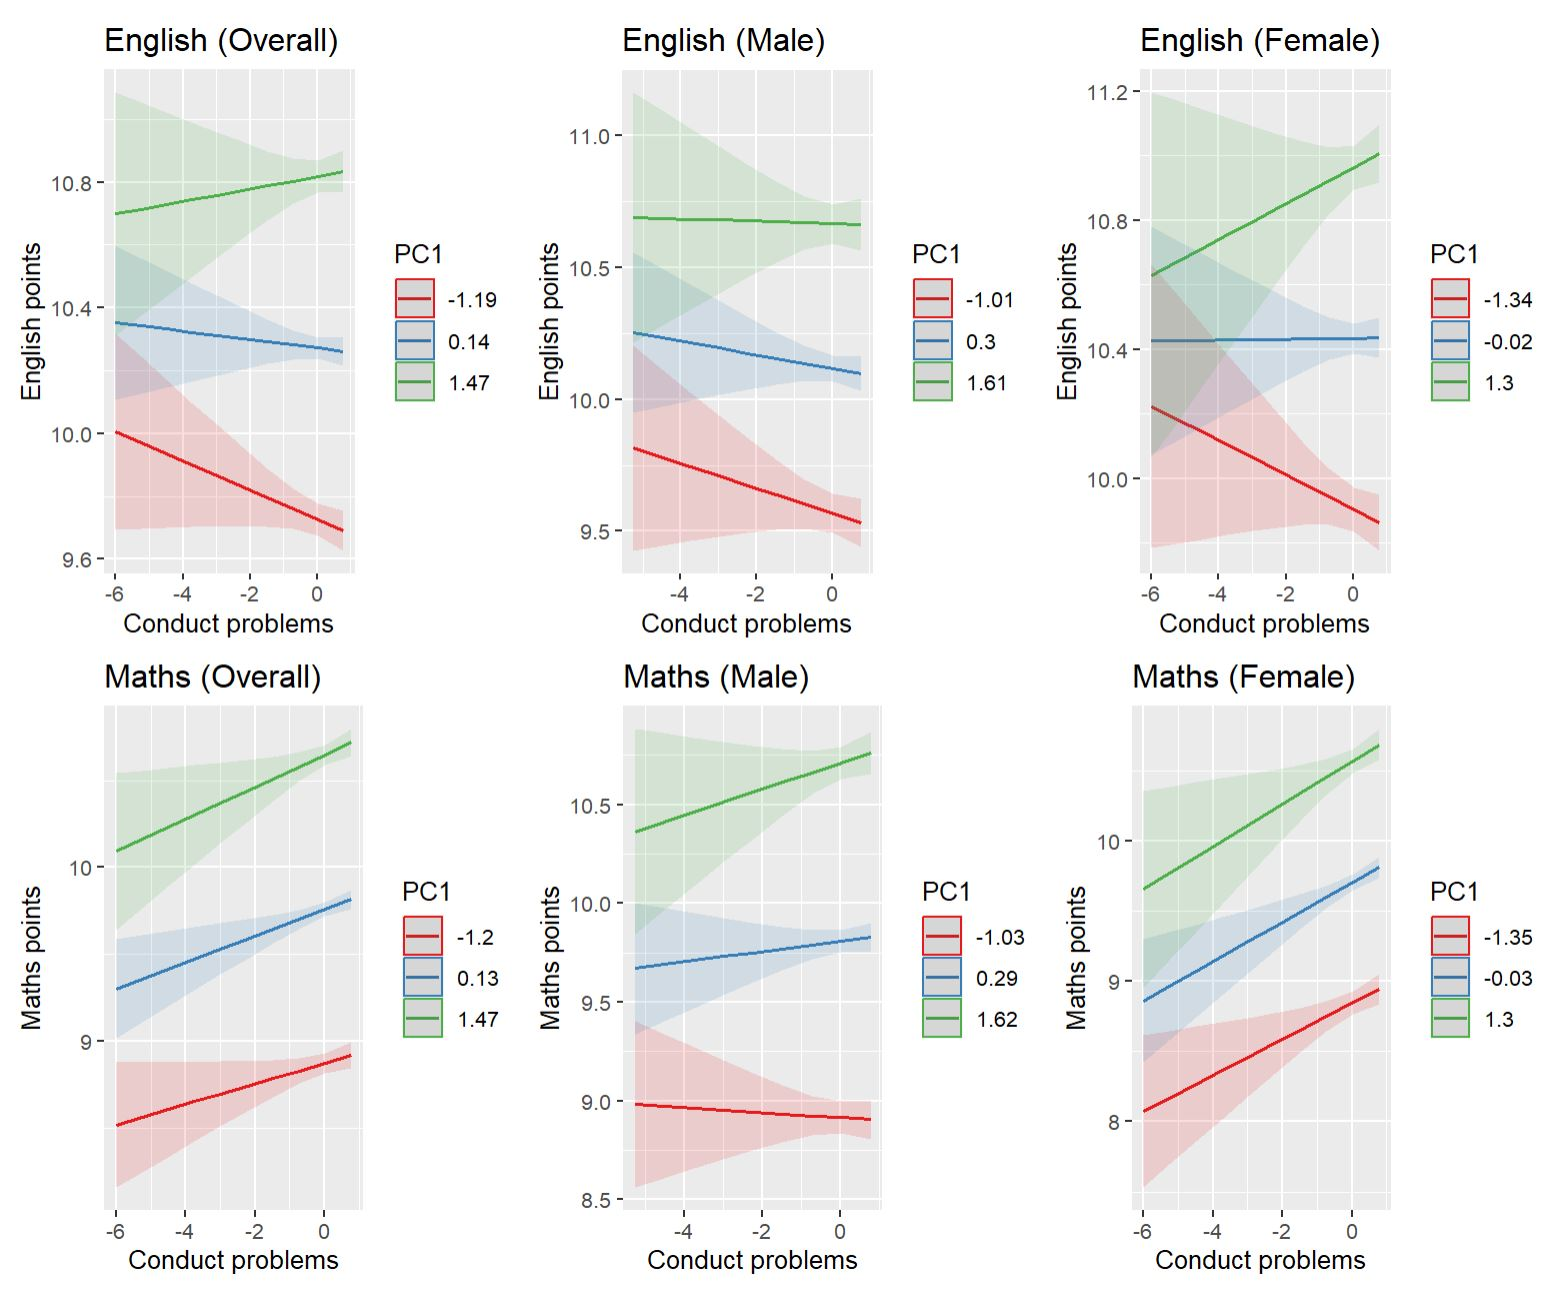
\includegraphics[width=1\linewidth]{AVE_SDQ_Conduct.JPG}
    \caption{The interaction between Conduct Problems and academic performance (English and Maths) stratified by gender and overall performance. The graphs above (Figure \ref{Fig1}) show three performance levels (proxied by the composite cognitive variable PC1): low (-1.19 to -1.35), average (around 0), and high (1.3 to 1.62). Conduct problems are plotted on the x-axis, with higher values indicating fewer problems. Both PC1 and Conduct problems have been standardized to have a mean = 0 and a standard deviation = 1. Maths and English scores are in their original scales.}
    \label{Fig1}
\end{figure*}

In Figure \ref{Fig1} we see that, overall, higher cognition scores correlate with better English performance for both genders. Students with fewer conduct problems tend to perform better in English, especially for high PC1 scores, and the effect is more pronounced for girls. Higher cognition scores also correlate with better Maths performance. For boys, conduct problems have little impact on Maths performance.
For girls, fewer conduct problems correlate with better Maths performance, especially for high cognition scores.

\begin{figure*}[ht] 
    \centering
    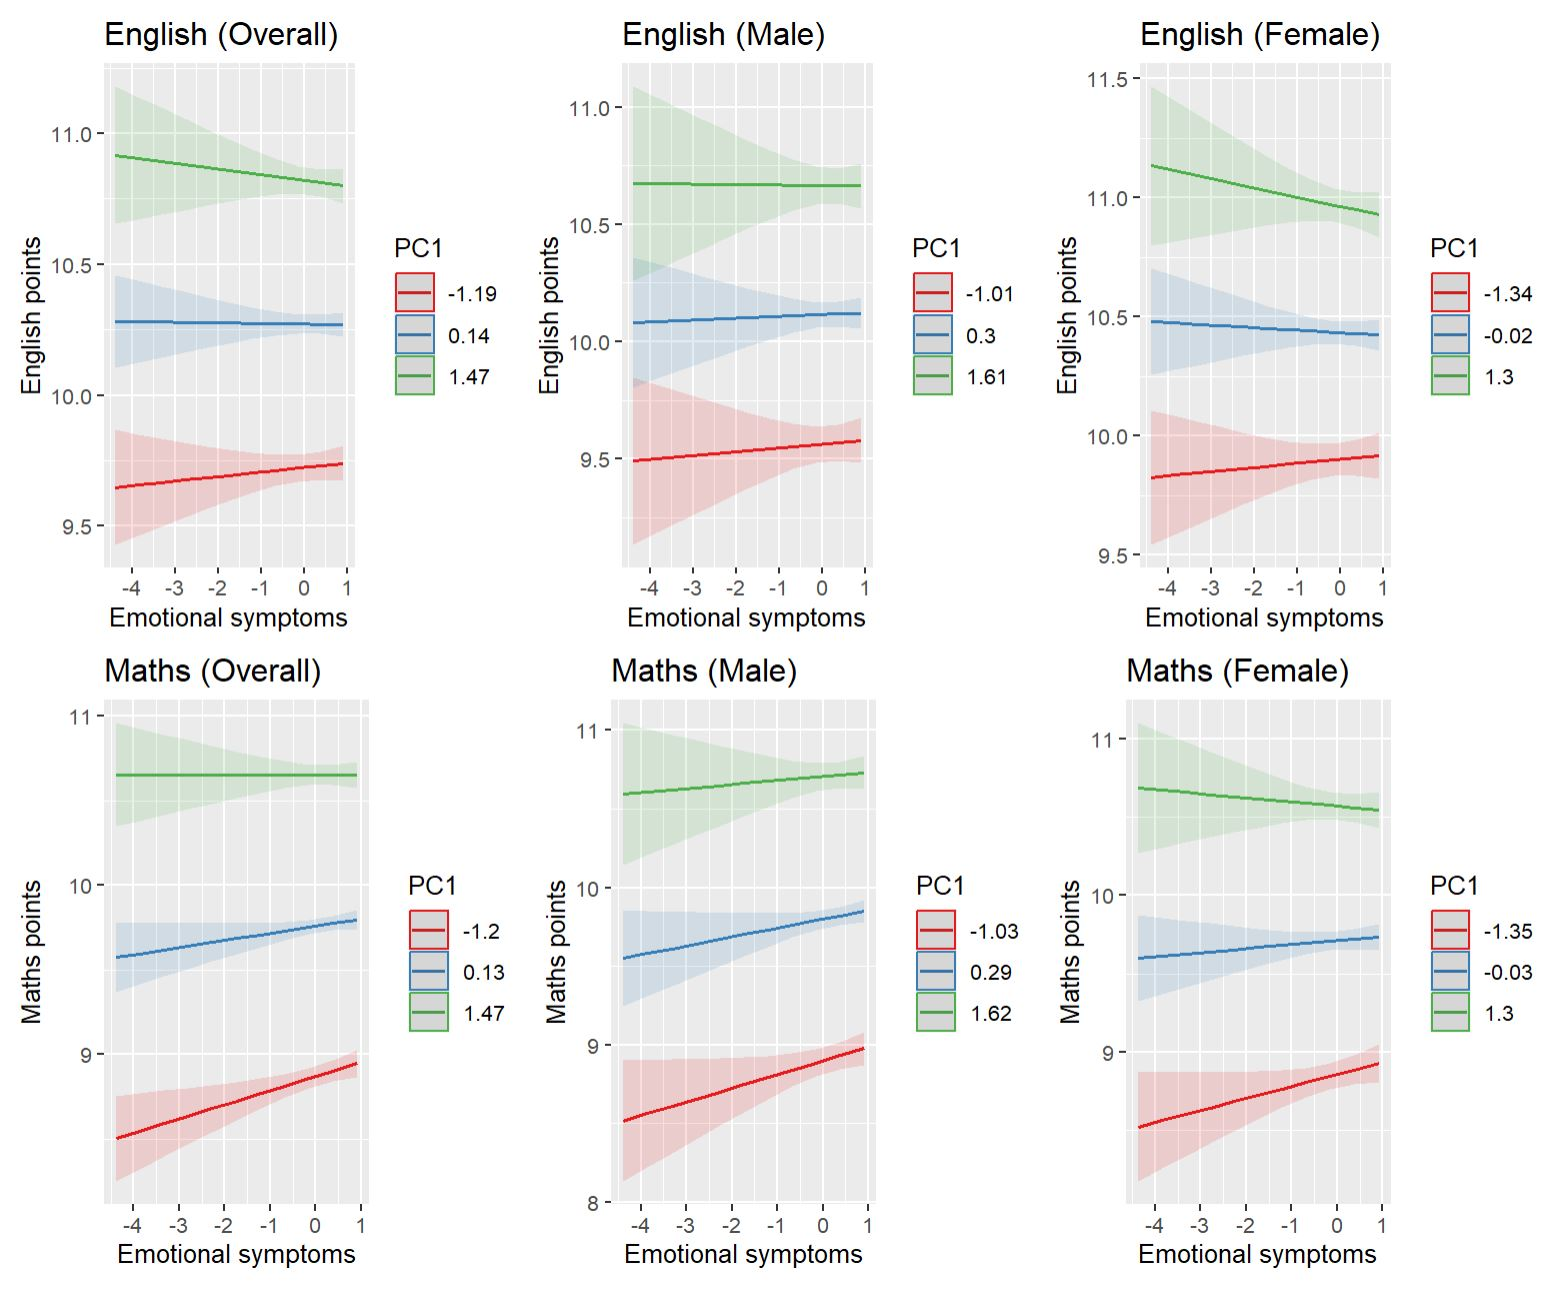
\includegraphics[width=1\linewidth]{AVE_SDQ_Emot.JPG}
    \caption{The interaction between Emotional symptoms and academic performance (English and Maths) stratified by gender and overall performance. The graphs above (Figure \ref{Fig2}) display three PC1 levels: low (red, varying between -1.2 and -1.35), average (blue, around 0), and high (green, varying between 1.3-1.62). Emotional symptoms are plotted on the x-axis, with higher values indicating fewer symptoms. Both PC1 and Emotional symptoms have been standardized to have a mean = 0 and a standard deviation = 1. Maths and English scores are in their original scales.}
    \label{Fig2}
\end{figure*}

 In Figure \ref{Fig2} we see that higher PC1 scores correlate with better English performance across both groups. The impact of emotional symptoms varies: for boys, fewer emotional symptoms slightly improve performance, especially for lower PC1 scores, while for girls, fewer emotional symptoms correlate with slightly lower performance, particularly for higher PC1 scores. Higher PC1 scores again correlate with better performance in Maths, and fewer emotional symptoms generally correlate with better Maths performance across both groups. The effect is more pronounced for boys, especially those with lower PC1 scores. Boys seem more affected by emotional symptoms in both subjects, showing steeper positive slopes as symptoms decrease.
Girls, on the other hand, show less variation in performance related to emotional symptoms, particularly in English.

\begin{figure*}[ht] 
    \centering
    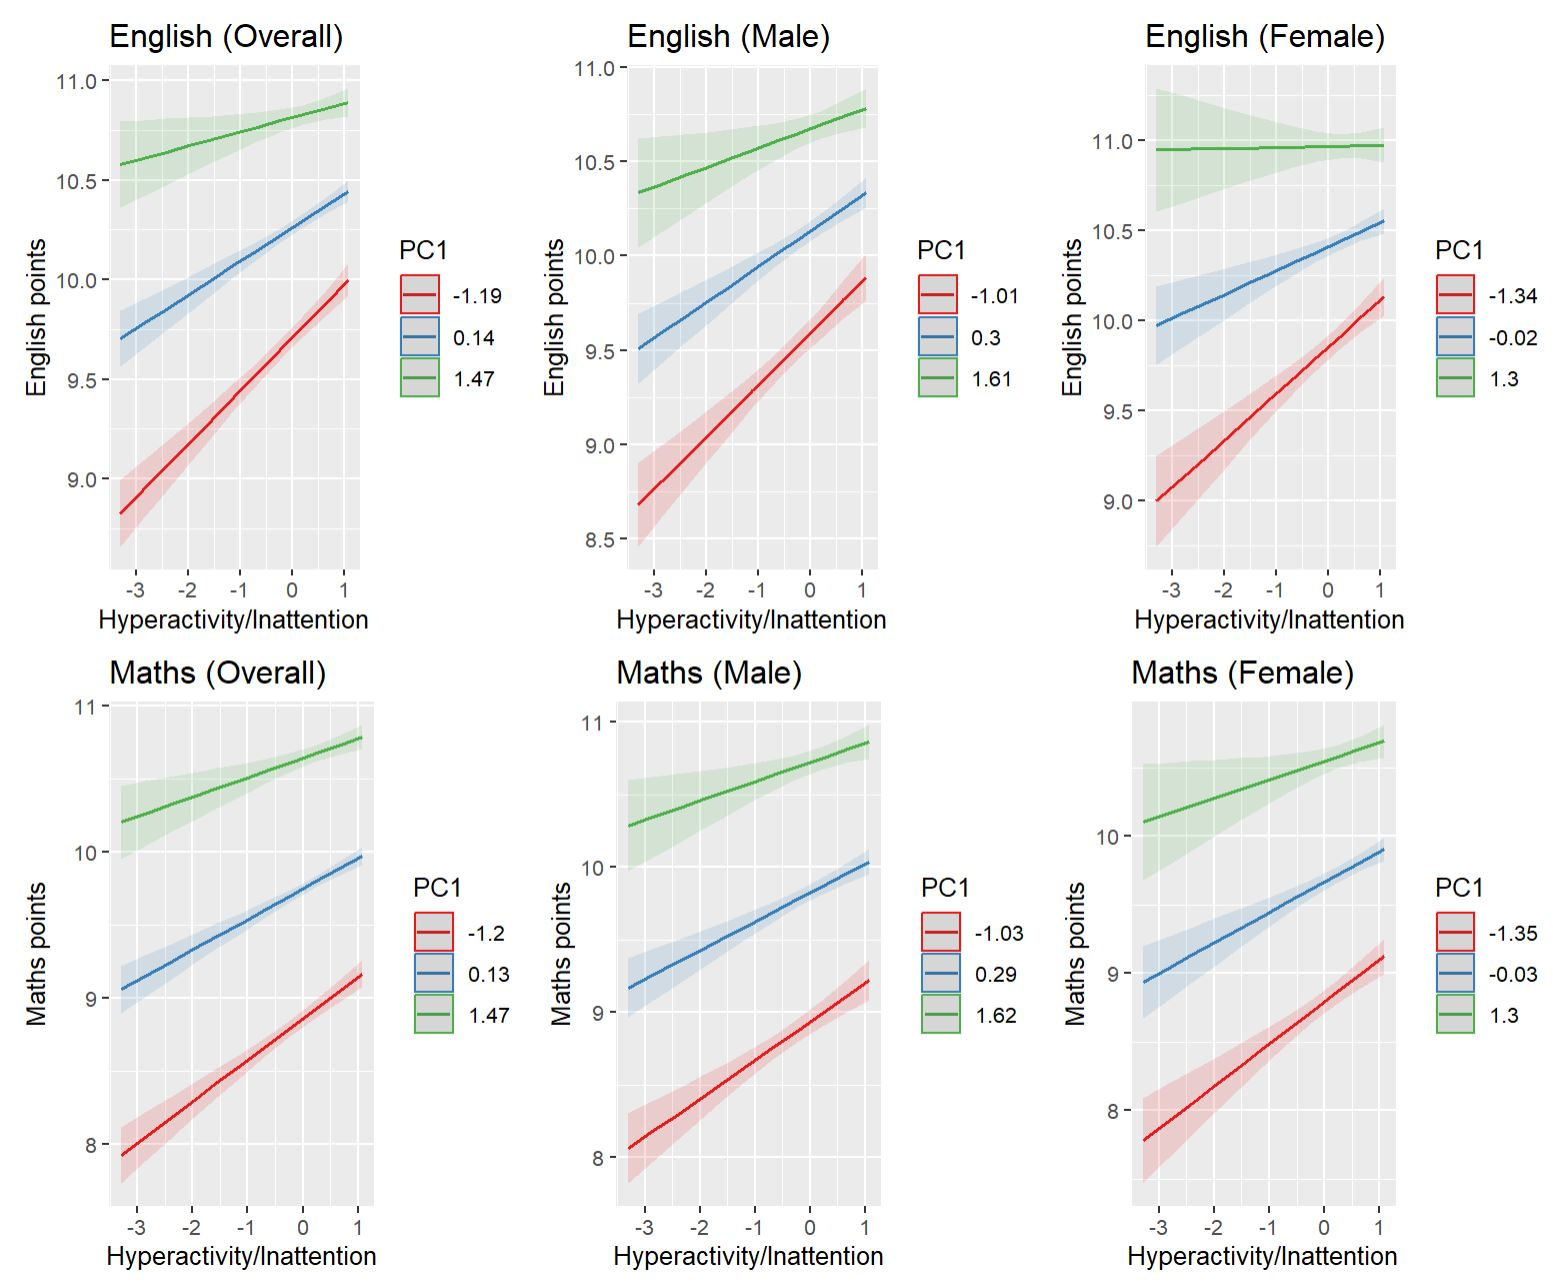
\includegraphics[width=1\linewidth]{AVE_SDQ_Hyper.JPG}
    \caption{The interaction between Hyperactivity/Inattention and academic performance (English and Maths) stratified by gender and overall performance. The graphs above (Figure \ref{Fig3}) show three PC1 levels: low (red, from -1.2 to -1.35), average (blue, around 0.13 to 0.3), and high (green, varying between 1.3 and 1.62). Hyperactivity/Inattention is plotted on the x-axis, with higher values indicating lower levels of Hyperactivity/Inattention. Both PC1 and Hyperactivity/Inattention have been standardized to have a mean = 0 and a standard deviation = 1. Maths and English scores are in their original scales.}
    \label{Fig3}
\end{figure*}

The relationship between Hyperactivity/Inattention and academic performance (Figure \ref{Fig3}) is relatively consistent across cognitive ability levels and genders, unlike the more varied patterns seen with other factors like emotional symptoms.
For both English and Maths, higher PC1 scores consistently correlate with better academic performance across both genders. Lower levels of Hyperactivity/Inattention (higher x-axis values) strongly correlate with better performance for all PC1 levels and groups. The slopes of the lines are always positive and steep, indicating a strong positive relationship between lower Hyperactivity/Inattention and academic performance. Boys show slightly steeper slopes in English, suggesting they may benefit more from reduced Hyperactivity/Inattention in this subject.
In Maths, the slopes are similar for both genders. The impact of Hyperactivity/Inattention appears more pronounced for students with lower PC1 scores (red lines), as evidenced by their steeper slopes.

\begin{figure*}[ht] 
    \centering
    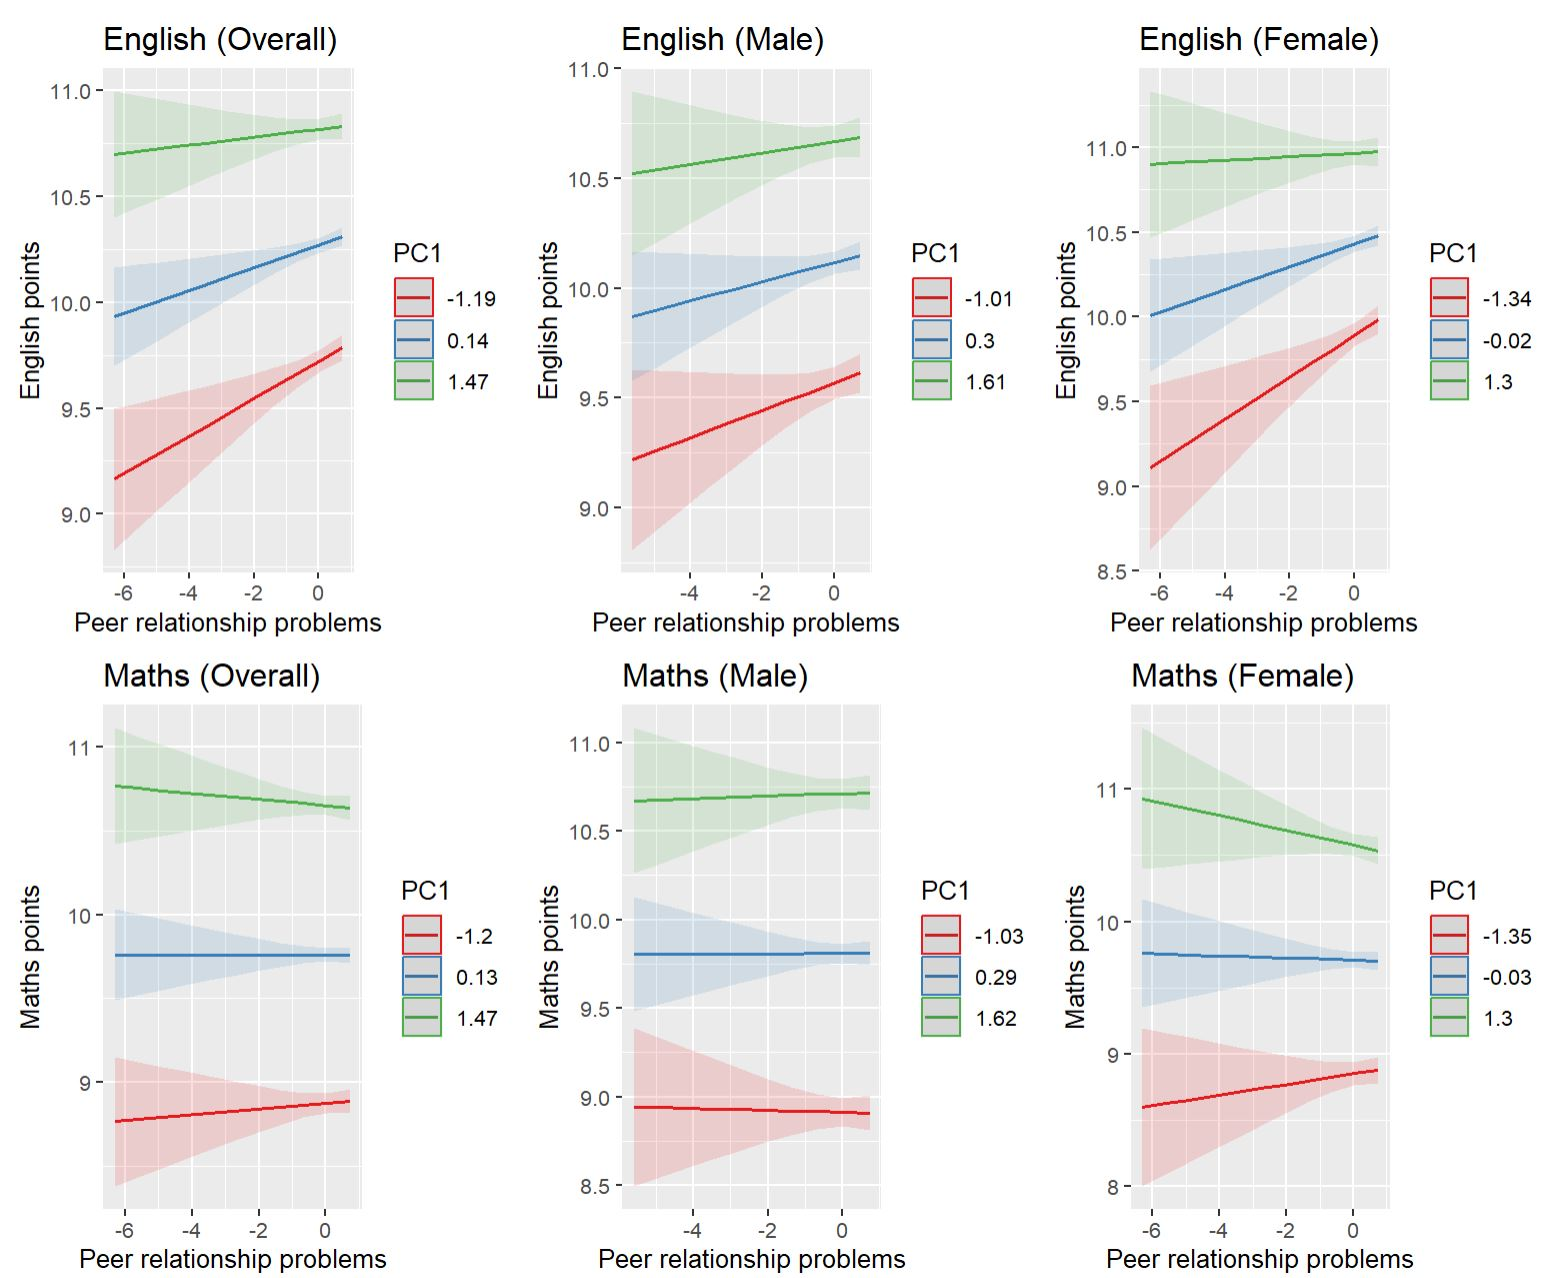
\includegraphics[width=1\linewidth]{AVE_SDQ_Peer.JPG}
    \caption{The interaction of Peer-relationship problems and academic performance (English and Maths) stratified by gender and overall performance. The graphs above (Figure \ref{Fig4}) show three PC1 levels: low (red, from -1.2 to -1.35), average (blue, from 0 to 0.3), and high (green, varying between 1.3 and 1.62). Peer-relationship problems are plotted on the x-axis, with higher values indicating fewer problems. Both PC1 and Peer-relationship problems have been standardized to have a mean = 0 and a standard deviation = 1. Maths and English scores are in their original scales.
}
    \label{Fig4}
\end{figure*}

Higher PC1 scores correlate with better English performance across both groups, and fewer Peer-relationship (Figure \ref{Fig4}) problems generally correlate with better English performance for both genders. The effect seems slightly stronger for students with lower PC1 scores. Higher PC1 scores again correlate with better performance in Maths. For boys, we can see a slight positive correlation between fewer problems and better performance in Maths, and for girls with high PC1 scores, fewer problems correlate with slightly lower Maths performance. In Maths, girls show more varied effects, particularly at higher PC1 levels. The relationship between Peer-relationship problems and academic performance is not uniform across cognitive ability levels or genders, and the impact seems more consistent for English across genders, which suggests possible non-obvious interactions. The effects of Peer-relationship problems appear less dramatic than those seen for Hyperactivity/Inattention in the previous graph.

In summary, cognitive ability (proxied by PC1) consistently correlates with higher academic performance across all subjects and measures. The four noncognitive variables have varying impacts on academic performance: Conduct problems generally show a negative correlation with performance, more pronounced in English and for girls; Emotional symptoms have mixed effects, with boys showing more sensitivity to these in both subjects; Hyperactivity/Inattention demonstrates the strongest and most consistent negative impact on performance across both genders and subjects; Peer-relationship problems have a moderate impact, more noticeable in English than in Math. Girls often show stronger correlations between noncognitive factors and performance in English, and boys tend to exhibit more consistent patterns across subjects. Interaction effects are evident: the impact of noncognitive factors often varies based on cognitive ability level (PC1), and students with lower cognitive abilities sometimes show stronger correlations between noncognitive factors and academic performance. When analysing the difference between subjects, we notice that English performance seems more sensitive to variations in noncognitive factors compared to Maths. Performance in Maths shows more varied and sometimes counterintuitive relationships with noncognitive factors, especially for high-ability students. The relationships between noncognitive factors and academic performance seem to be more intricate and non-uniform than previously expected, which suggests that interventions and support strategies may need to be tailored based on cognitive ability, gender, and specific subject areas. Of all noncognitive variables of the SDQ scale examined, addressing Hyperactivity/Inattention might yield the most consistent benefits for academic performance across all groups.

\subsection{TIPI}

\begin{figure*}[ht] 
    \centering
    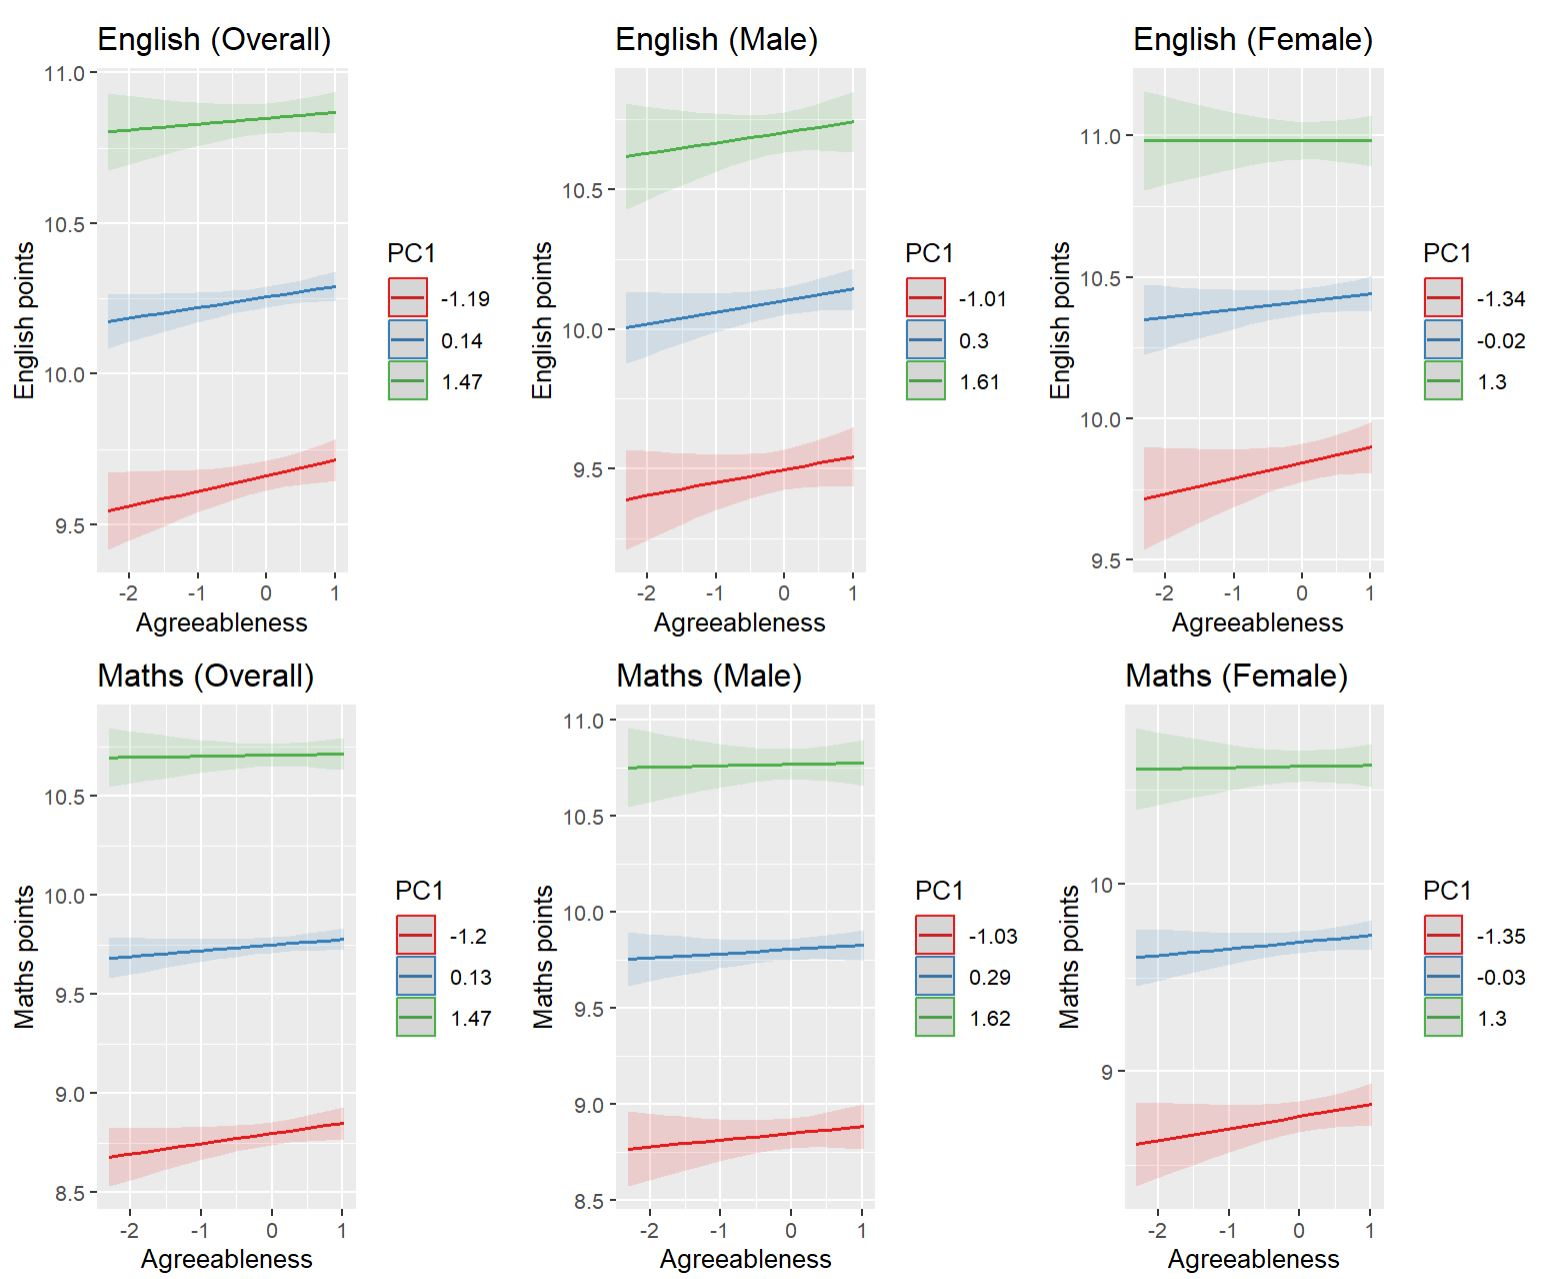
\includegraphics[width=1\linewidth]{AVE_TIPI_Agree.JPG}
    \caption{The interaction between Agreeableness and academic performance (English and Maths) stratified by gender and overall performance. The graphs above (Figure \ref{Fig5}) show three PC1 levels: low (red, from -1.2 to -1.35), average (blue, from 0 to 0.3), and high (green, varying between 1.3 and 1.62). Agreeableness is plotted on the x-axis, ranging from -2 to 1, with higher values indicating higher Agreeableness. Both PC1 and Agreeableness have been standardized to have a mean = 0 and a standard deviation = 1. Maths and English scores are in their original scales.
}
    \label{Fig5}
\end{figure*}

Agreeableness (Figure \ref{Fig5}) shows a generally positive, but modest, relationship with academic performance. This effect is more pronounced for English than Maths and varies somewhat by gender and cognitive ability level. The impact of agreeableness appears less dramatic than some other noncognitive factors we've examined previously. The relationship between Agreeableness and academic performance appears more consistent across cognitive ability levels compared to some other factors, though still showing some variation. Higher PC1 scores always correlate with better English and Maths performance across all groups. Increased Agreeableness generally shows a slight positive correlation with English performance for all groups. The effect appears slightly stronger for boys, especially those with lower PC1 scores. The impact of Agreeableness on Maths performance is less pronounced than for English, and there is a slight positive correlation between agreeableness and Maths performance, more noticeable for girls and those with lower PC1 scores. The slopes for agreeableness are generally less steep compared to some other noncognitive factors we've seen (e.g., Hyperactivity/Inattention), suggesting a more modest impact on academic performance.

\begin{figure*}[ht] 
    \centering
    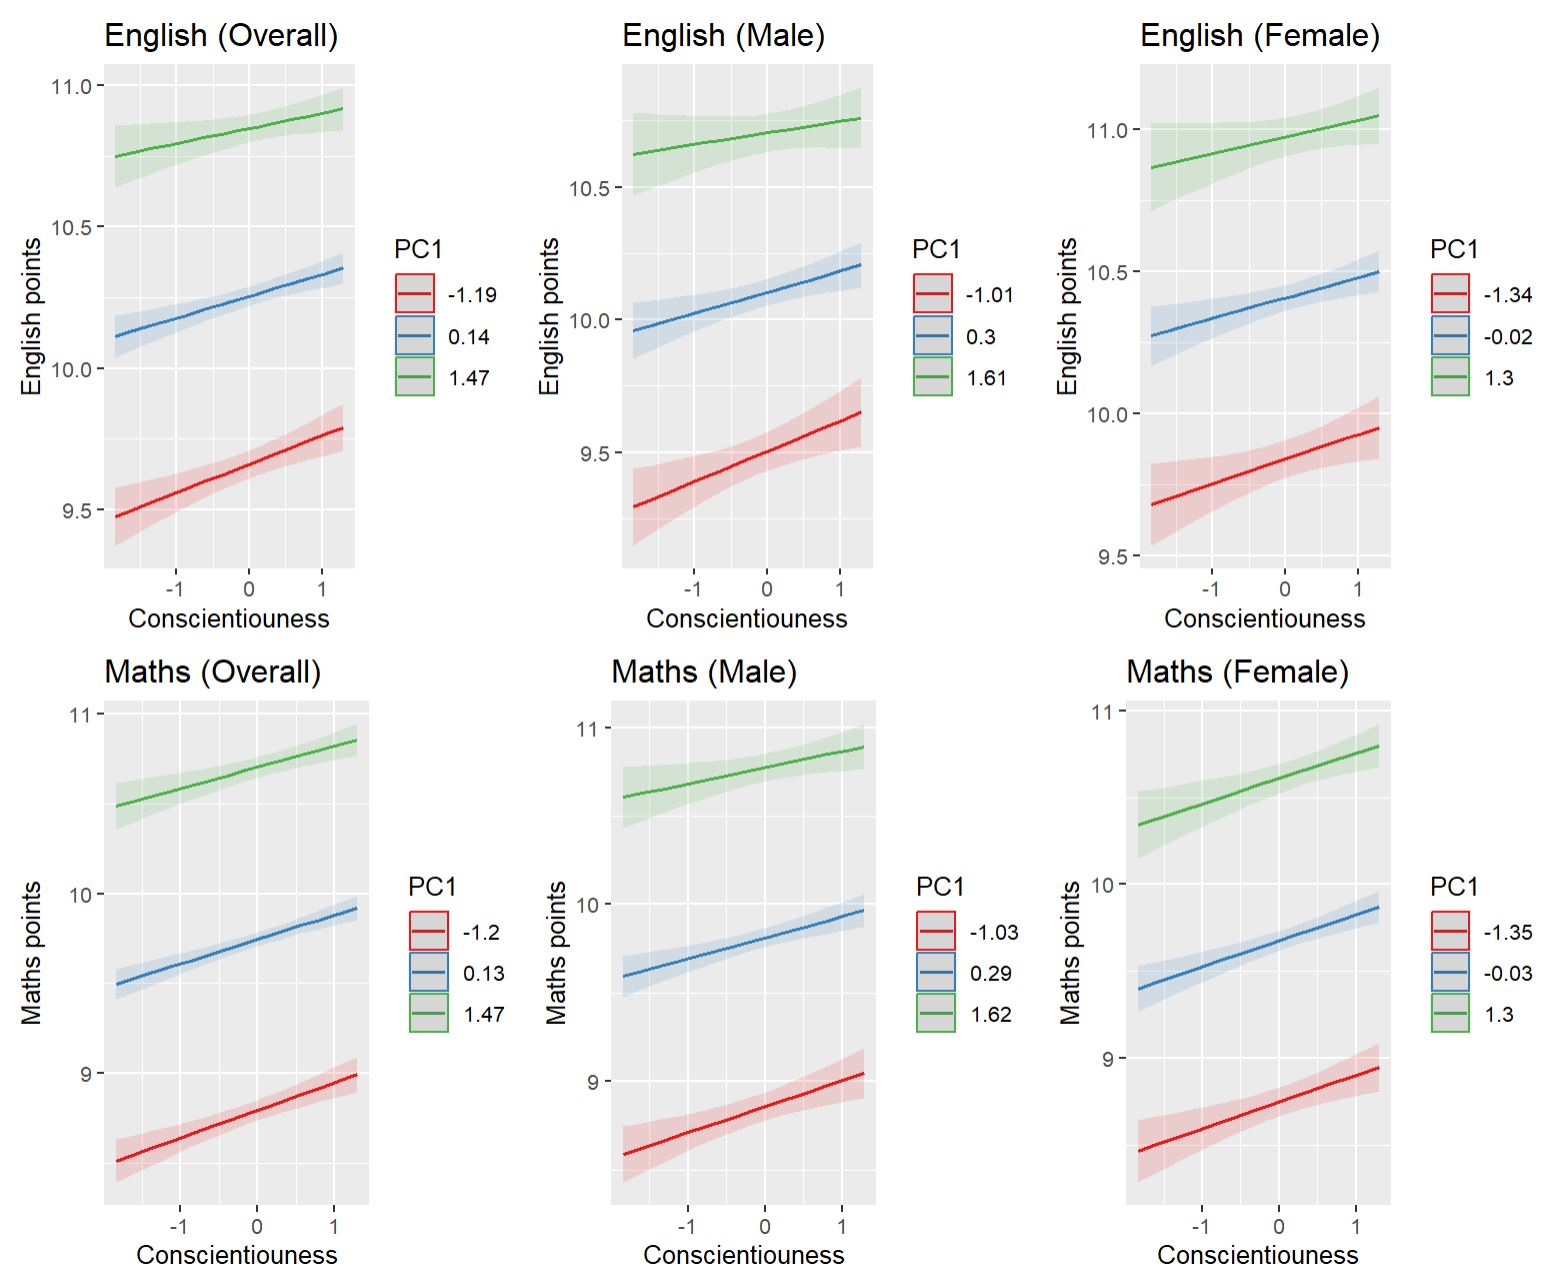
\includegraphics[width=1\linewidth]{AVE_TIPI_Cons.JPG}
    \caption{The interaction between Conscientiousness and academic performance (English and Maths) stratified by gender and overall performance. The graphs above (Figure \ref{Fig6}) display three PC1 levels: low (red, from -1.1 to -1.35), average (blue, around 0 to 0.3), and high (green, varying between 1.3 to 1.62). Conscientiousness is plotted on the x-axis, ranging from -1 to 1, with higher values indicating higher Conscientiousness. Both PC1 and Conscientiousness have been standardized to have a mean = 0 and a standard deviation = 1. Maths and English scores are in their original scales.}
    \label{Fig6}
\end{figure*}

Conscientiousness (Figure \ref{Fig6}) shows a generally positive relationship with academic performance across all groups. This effect is consistent for both English and Maths and is relatively similar for boys and girls. The impact of Conscientiousness seems more pronounced than a few previous noncognitive variables, as evidenced by steeper slopes in most cases. We see that higher PC1 scores consistently correlate with better English and Maths performance across all groups.
Increased Conscientiousness shows a positive correlation with both English and Maths performance for all groups. The effect of Conscientiousness appears slightly stronger for English than for Maths, and it is relatively consistent across genders, with only minor variations. The positive effect of Conscientiousness is evident across all PC1 levels, but the slopes are steepest for the high PC1 group (green lines).

\begin{figure*}[ht] 
    \centering
    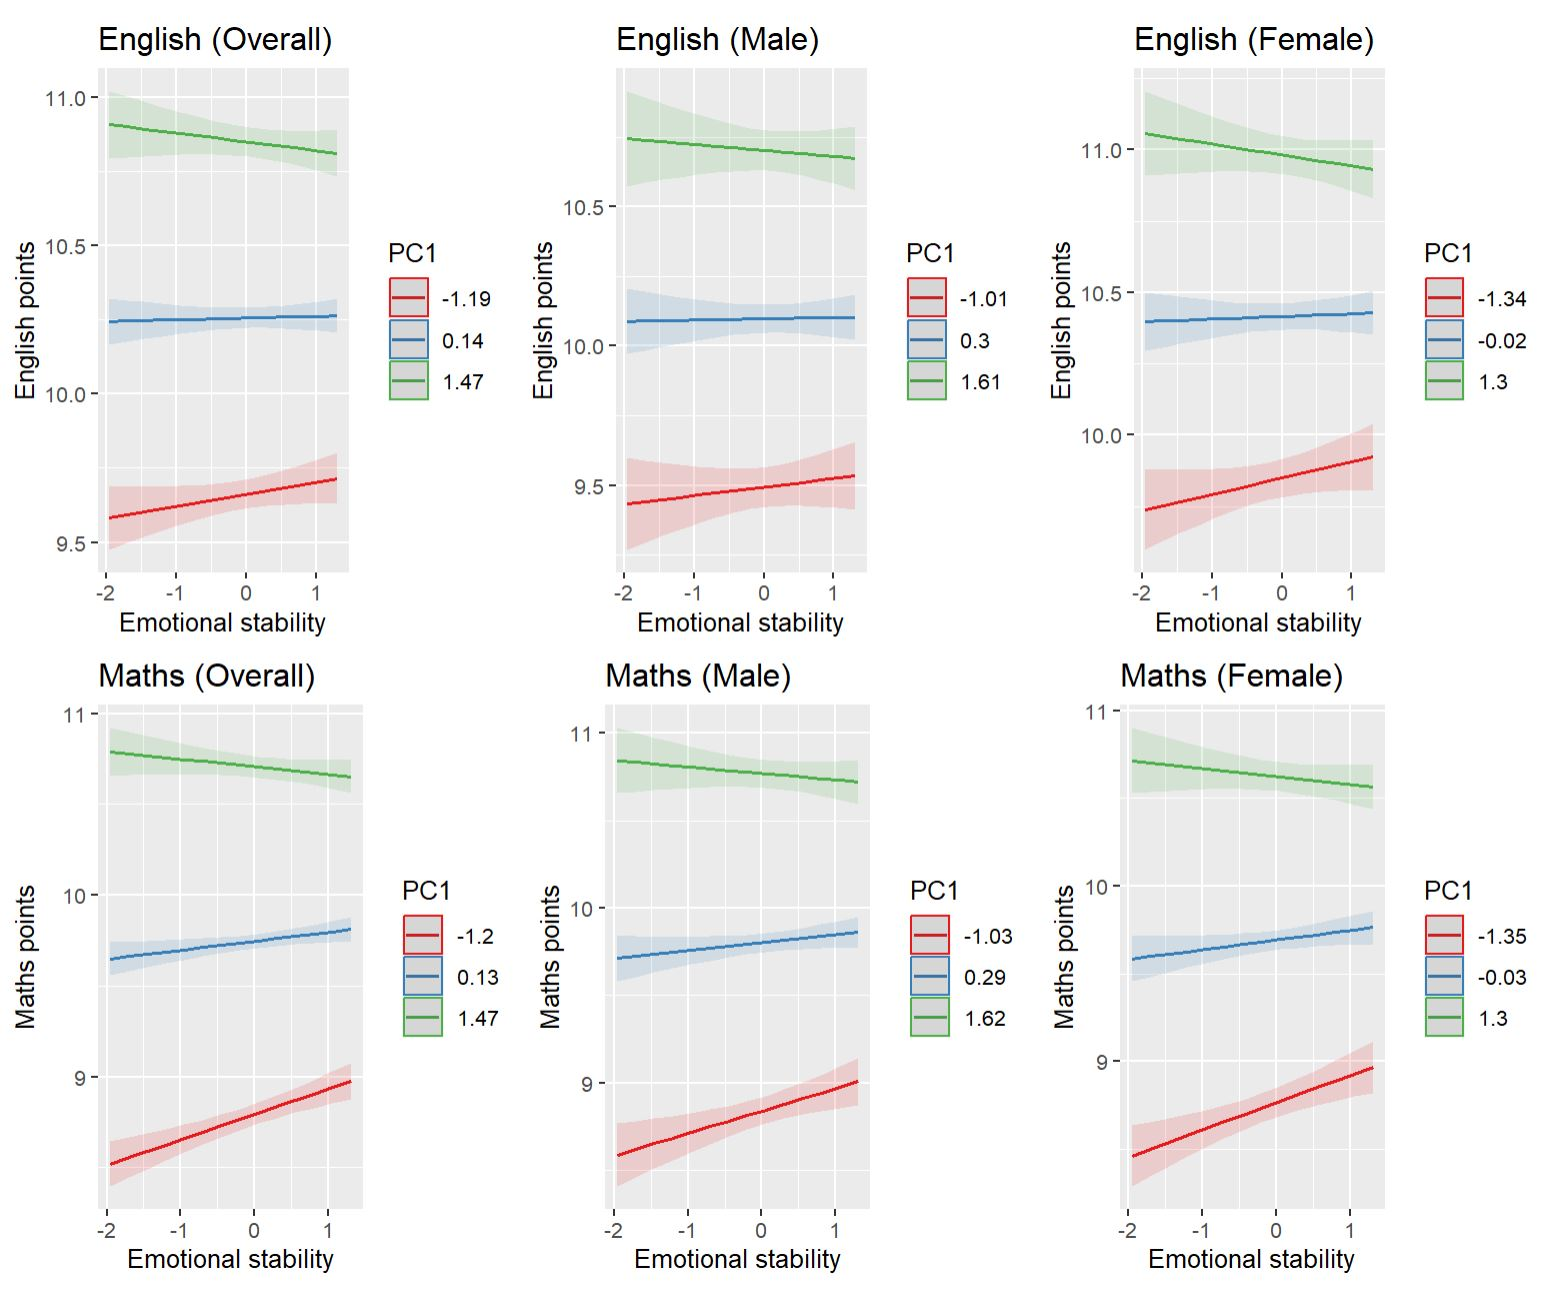
\includegraphics[width=1\linewidth]{AVE_TIPI_Emot.JPG}
    \caption{The interaction between Emotional stability and academic performance (English and Maths) stratified by gender and overall performance. The graphs above (Figure \ref{Fig7}) display three PC1 levels: low (red, from -1.01 to -1.35), average (blue, from -0.03 to 0.3), and high (green, varying from 1.3 to 1.62). Emotional stability is plotted on the x-axis, ranging from -2 to 1, with higher values indicating higher levels of Emotional stability. Both PC1 and Emotional stability have been standardized to have a mean = 0 and a standard deviation = 1. Maths and English scores are in their original scales.}
    \label{Fig7}
\end{figure*}

Emotional stability (Figure \ref{Fig7}) shows a positive relationship with academic performance, particularly for lower PC1 groups. For English, the effect is more pronounced for girls, especially those with lower PC1 scores. For Maths, the positive relationship is stronger compared to English, with steeper slopes across all groups. The impact of emotional stability appears slightly stronger for girls in both subjects. Again, higher PC1 scores persistently correlate with better performance, but the slopes are steepest for the low PC1 group.

\begin{figure*}[ht] 
    \centering
    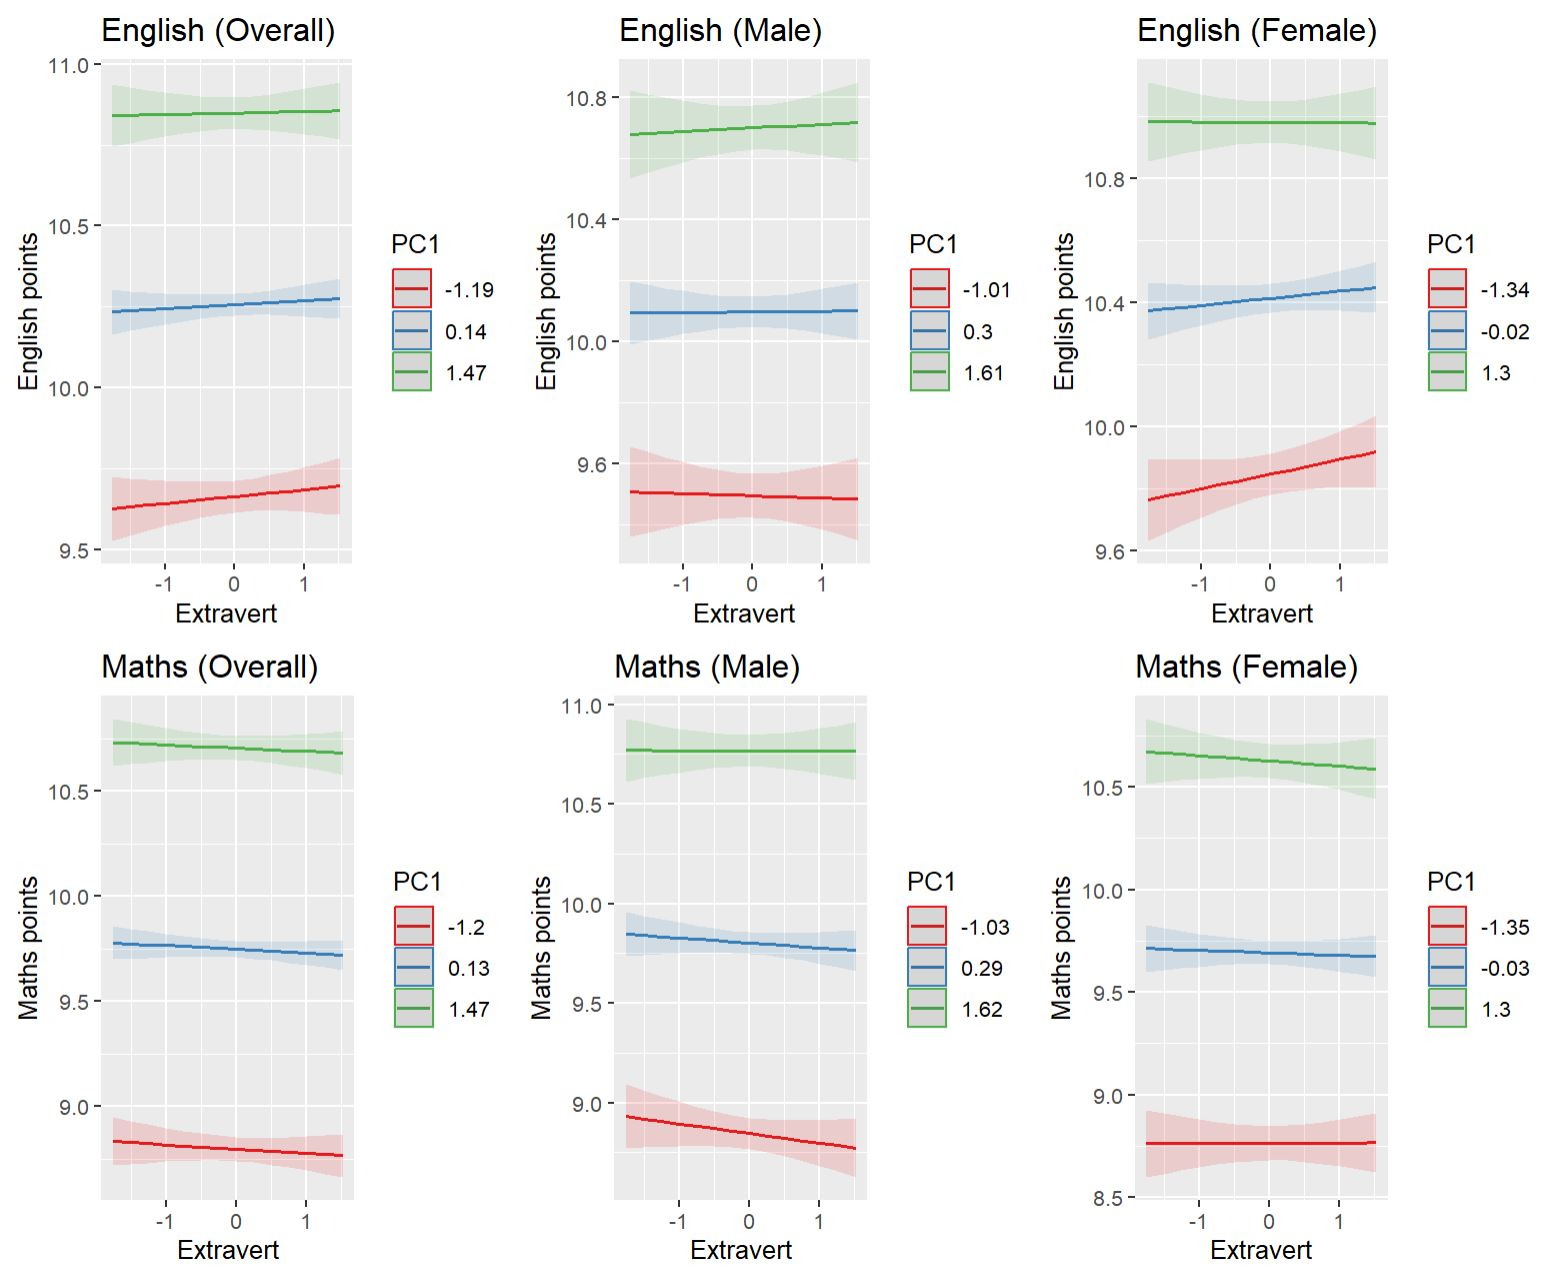
\includegraphics[width=1\linewidth]{AVE_TIPI_Extra.JPG}
    \caption{The interaction between Extroversion and academic performance (English and Maths) stratified by gender and overall performance. The graphs above (Figure \ref{Fig8}) display three PC1 levels: low (red, from -1.01 to -1.35), average (blue, around -0.03 to 0.3), and high (green, varying from 1.3 to 1.62). Extroversion is plotted on the x-axis, ranging from -1 to 1, with higher values indicating higher levels of Extroversion. Both PC1 and Extroversion have been standardized to have a mean = 0 and a standard deviation = 1. Maths and English scores are in their original scales.}
    \label{Fig8}
\end{figure*}

Extroversion (Figure \ref{Fig8}) shows a weak and inconsistent relationship with academic performance. For English, there is a slight positive trend for girls, but minimal effect for boys. For Maths, on the other hand, a slight negative trend is observed, more noticeable for boys and those with higher PC1 scores. Girls show a more positive (or less negative) relationship between extroversion and performance compared to boys, and higher PC1 scores correlate with better performance, but the impact of extroversion varies across PC1 levels.

\begin{figure*}[ht] 
    \centering
    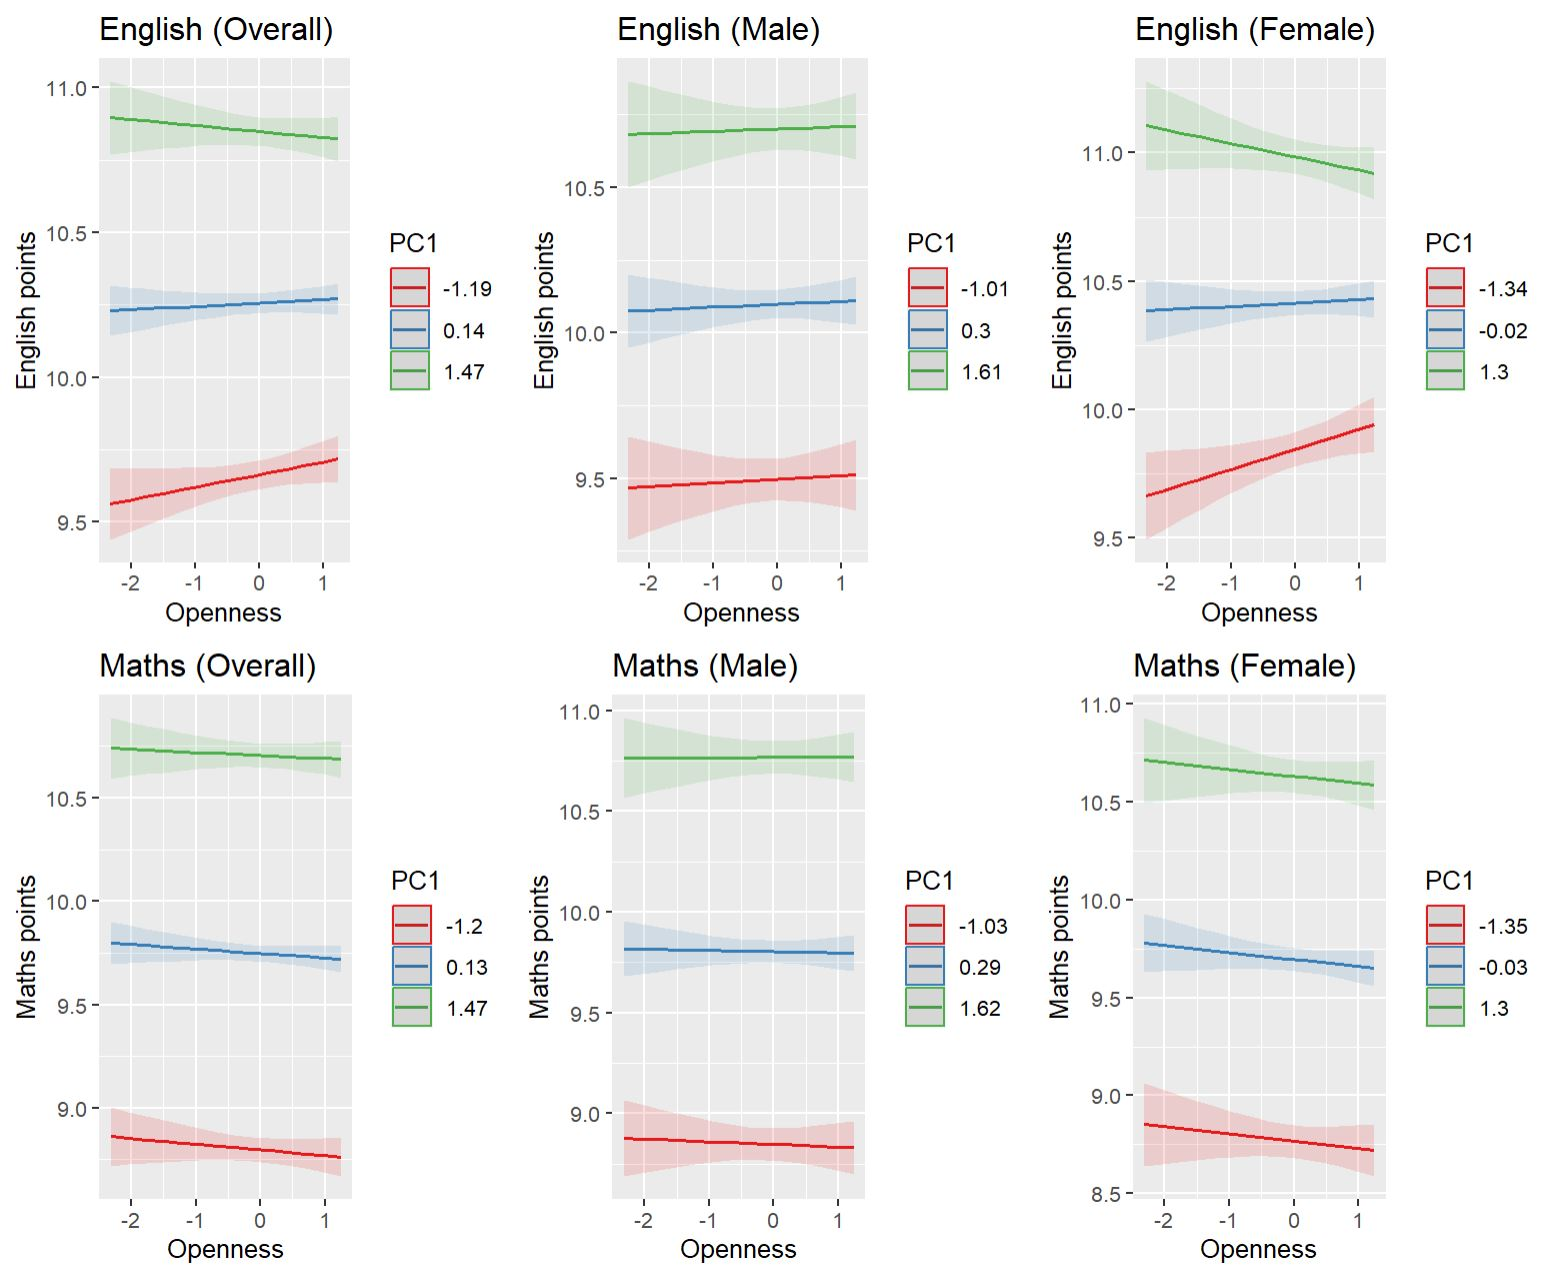
\includegraphics[width=1\linewidth]{AVE_TIPI_Open.JPG}
    \caption{The interaction between Openness and academic performance (English and Maths) stratified by gender and overall performance. The graphs above (Figure \ref{Fig9}) display three PC1 levels: low (red, from -1.01 to -1.35), average (blue, varying between -0.03 and 0.3), and high (green, around 1.3 to 1.62). Openness is plotted on the x-axis, ranging from -2 to 1, with higher values indicating higher levels of Openness. Both PC1 and Openness have been standardized to have a mean = 0 and a standard deviation = 1. Maths and English scores are in their original scales.}
    \label{Fig9}
\end{figure*}

Openness (Figure \ref{Fig9}) shows a mixed relationship with academic performance, varying by subject and gender. For English, a slightly positive trend is observed, more pronounced for girls. For Maths, a subtle negative trend is seen across all groups, more noticeable for those with higher PC1 scores. Girls show a more positive (or less negative) relationship between Openness and performance compared to boys, and higher PC1 scores correlate with better performance, but the impact of Openness is more pronounced for higher PC1 groups, especially in Maths.

We see, repetitively, that higher PC1 scores correlate with better performance across all traits and subjects, and that we observe differences in how traits relate to academic performance. Agreeableness: Modest positive effect, stronger for English than Math. Conscientiousness: Consistent positive effect across subjects and genders. Emotional stability: Positive effect, stronger for lower PC1 groups and slightly more for girls.
Extroversion: Weak and inconsistent effects, slightly positive for girls in English, slightly negative for boys in Math. Openness: Mixed effects, slightly positive for English (especially girls), slightly negative for Math. Trait effects often differ between English and Maths performance, with some traits (e.g., Conscientiousness) showing more consistent effects across subjects than others. In terms of effect magnitude, Conscientiousness appears to have the strongest overall positive effect, with other traits showing more modest or variable impacts on academic performance. The impact of personality traits often varies across different PC1 levels, and some traits show stronger effects for lower PC1 groups, while others are more pronounced for higher PC1 groups.

\section{Explaining the gender achievement-gap}

\begin{figure*}[ht] 
    \centering
    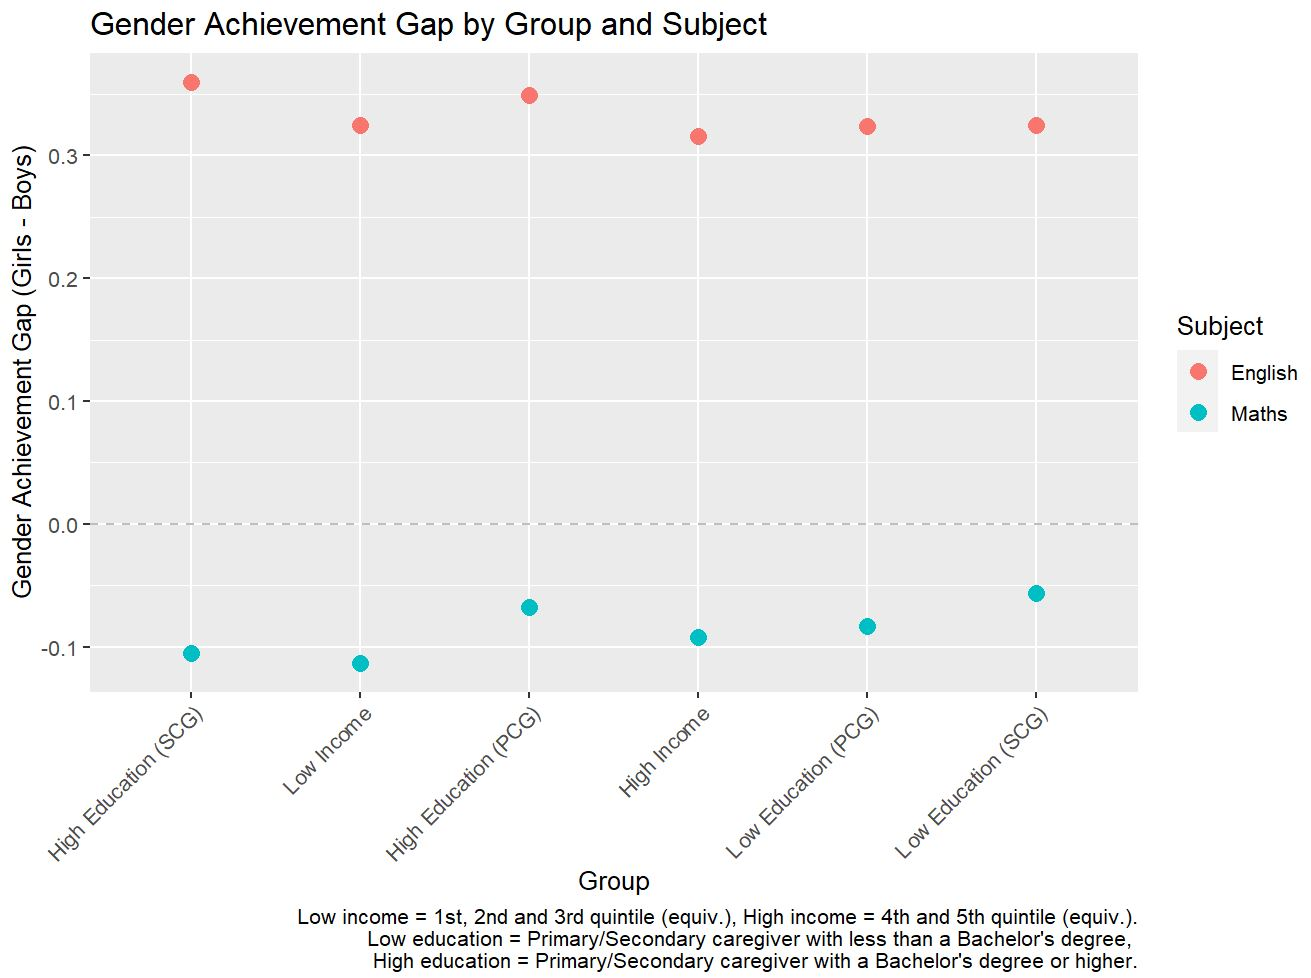
\includegraphics[width=1\linewidth]{Gender_gap_by_group.JPG}
    \caption{Gender Achievement Gap by Socioeconomic Group and Subject. This plot illustrates the gender achievement gap in English and Maths across different socioeconomic groups. The y-axis represents the gender gap, calculated as girls' mean score in the Junior Cert minus boys' mean score. Positive values indicate girls outperform boys, while negative values show boys outperform girls. The x-axis categories represent different income and parental education levels. Points above the dashed line ($y=0$) indicate a female advantage, while points below indicate a male advantage.}
    \label{fig:OBDecompGroup}
\end{figure*}

While the regression results from the previous chapter helped us understand how cognition and noncognition affect test scores, it does not provide a full picture of the more nuanced characteristics of the sample. Due to the negative coefficient for Male, it was necessary to break down the sample into a few sub-samples. I began by creating two separate datasets, one for English scores and one for Maths scores. In each dataset, I included mean scores for girls and boys across different socioeconomic groups. These groups were based on household income levels (low income: 1st, 2nd, and 3rd quintiles; high income: 4th and 5th quintiles) and parental education levels (low education: less than a Bachelor's degree; high education: Bachelor's degree or higher). Next, I calculated the gender achievement gap for each group and subject. To do this, I subtracted the boys' mean score from the girls' mean score for each socioeconomic group in both English and Maths. Raw results are presented in Tables \ref{TableGenderAchievementGapMaths} and \ref{TableGenderAchievementGapEnglish}. This gave me a single value representing the gender gap, where a positive number meant girls outperformed boys, and a negative number meant boys outperformed girls. That is represented in Figure \ref{fig:OBDecompGroup}. Results show that across all income and education groups, boys outperform girls in Maths, and girls outperform boys in English. The achievement gap is also always smaller (in absolute values) in Maths than in English. 

For Maths, the gender achievement gap is largest in the low-income group and smallest in the primary caregiver high-education group (where the mother - for the majority of the sample - has at least a Bachelor's degree). Higher income and higher education levels, for both caregivers, are associated with better performance overall in Maths for both genders. The income effect (the difference in gender gaps - differences between boys' and girls' mean scores - between groups categorized by income level) is lower than the education effects (the difference, or gap, in means between groups - boys and girls - characterized by education levels of the caregivers), which suggests that parental education (especially of the secondary caregiver, which for the majority of the sample is the father) have a stronger influence in Maths performance than household income. Interestingly, household income and primary caregiver's education appear to narrow the achievement gap for Maths, while secondary caregiver's education widens it. Having a secondary caregiver with at least a bachelor's degree seem to have a positive effect on girls' Maths performance seeing that they are the group with the highest mean. The gender gap is wider in the high education secondary caregiver group compared to the low education secondary caregiver group, however, both girls and boys perform better in the high education secondary caregiver group, with girls showing a larger improvement compared to boys. This means that while the gender gap widens, girls still benefit from having a highly educated secondary caregiver, just not quite as much as boys do in terms of Maths performance. The gender ratios (the ratio between Girls Mean and Boys Mean) are all a bit below 1, which means that boys always perform better than girls across all groups in Maths, but the across-group difference is relatively small. The highest gender ratio in Maths is in the low education secondary caregiver group, meaning that the gender gap is smallest when the secondary caregiver has lower education levels. 

For English, the largest gender gap is observed in the group where the secondary caregiver has at least a Bachelor's degree, and the smallest in the high-income group. As with Maths, a higher household income is associated with better performance in English for both genders, and the gender gap decreases in higher income groups, which suggests that increased income can have a marginally stronger and positive effect on boys' performance. Higher education levels for both primary and secondary caregivers are associated with larger gender gaps, which indicates that girls might benefit more in English from having more educated caregivers.

For English, the gender ratios are all above 1, confirming girls' superior performance. The gender ratio is highest in the high education secondary caregiver group for English, mirroring the finding that this group also has the largest gender gap. This suggests that while higher secondary caregiver education benefits both genders in English, it appears to disproportionately benefit girls.

Overall, both income and caregiver education levels have a positive effect on Maths and English performances, and the effects of caregivers' education are stronger than the income effects, especially for Maths. 

The findings from this analysis have implications for our understanding of human capital formation and the economics of education. The persistent gender gaps in academic performance, particularly the male underperformance in English and female underperformance in Maths suggest potential inefficiencies in human capital accumulation. These gaps may lead to suboptimal educational and career choices, potentially affecting labor market outcomes and overall economic productivity \parencite{altonji1999race}.

The strong influence of cognitive factors on academic performance further emphasizes the importance of early skill formation, as championed by \textcite{heckman2006skill}. The differences in returns to cognitive and noncognitive skills between genders suggest that there might be gender-specific patterns in the production function of human capital, which could have implications for understanding wage differentials and occupational segregation later in the labor market \parencite{blau2017gender}.

Also the finding that socioeconomic and school-related factors mediate some of the gender differences in cognitive skills highlights the role of family background and educational inputs in shaping academic outcomes. This aligns with the literature on intergenerational transmission of human capital and the production function of cognitive and noncognitive skills \parencite{cunha2007technology}.

The varying gender gaps across different income and education levels suggest that the relationship between socioeconomic status and academic achievement is complex and potentially non-linear. This finding contributes to the ongoing debate about the relative importance of nature versus nurture in determining educational outcomes \parencite{sacerdote2011nature}.

The gender gaps in academic performance observed may have significant long-term economic consequences, particularly in terms of occupational segregation and wage differentials in the labor market. The underperformance of boys in English and girls in Maths could potentially lead to gender-based sorting into different educational tracks and, subsequently, into different occupations. This aligns with the theory of comparative advantage in occupational choice \parencite{rosen1978substitution}, where individuals select occupations based on their relative strengths.

As an example, the superior performance of girls in English might lead to their overrepresentation in humanities and social sciences, while boys' better performance in Maths could result in their dominance in STEM fields. This occupational segregation does have substantial implications for the labor market and the economy as a whole. \textcite{blau2017gender} argue that occupational segregation is a major contributor to the gender wage gap, as female-dominated occupations often pay less than male-dominated ones, even when controlling for skill levels and job characteristics.

Also, if these academic performance gaps persist into adulthood, they could contribute to skill differentials between men and women in the labor force. Given the increasing importance of both quantitative and communication skills in the modern economy \parencite{deming2017growing}, gender-based skill gaps would then lead to inefficient allocation of talent and reduced overall productivity.

My findings also relate to theories of statistical discrimination in labor markets \parencite{phelps1972statistical}. If employers believe that these gender differences in academic performance reflect underlying differences in skills or abilities, they might use gender as a proxy for productivity in hiring and promotion decisions. For example, an employer might be more inclined to hire a man for a maths-intensive job based on the average performance gap, even if the specific woman applicant is equally or more qualified, which then triggers a snowball effect, that could lead to a self-fulfilling prophecy where women, anticipating discrimination, invest less in maths skills, thus perpetuating the gap.

I have to note that these potential long-term consequences are speculative and based on the assumption that early academic performance gaps persist and translate into labor market outcomes. Longitudinal studies tracking individuals from school to the labor market would be necessary to confirm these hypotheses. 

\begin{table}[htbp]
\centering
\caption{Gender Achievement Gap in Maths by Socioeconomic Factors. This table presents mean Junior Certificate Maths scores for girls and boys across different income and parental education groups. Low-income levels are equivalent to the 1st, 2nd, and 3rd quintiles, while High-income accounts for the 4th and 5th quintiles. Parental education levels are separated by Low education (less than a Bachelor's degree) and High education (a Bachelor's degree or higher) for Primary caregiver (PCG) and Secondary Caregiver (SCG). It shows gender gaps (girls' mean minus boys' mean), overall mean scores, and gender ratios (girls' mean divided by boys' mean) for each group. Socioeconomic effects are calculated as the difference between high and low categories for each factor.}
\begin{tabular}{lccccc}
\hline
\multirow{2}{*}{Group} & \multicolumn{2}{c}{Mean Scores} & \multicolumn{3}{c}{Differences and Ratios} \\
\cmidrule(lr){2-3} \cmidrule(lr){4-6}
 & Girls Mean & Boys Mean & Gender Gap & Overall Mean & Gender Ratio \\
\hline
\multicolumn{6}{l}{\textbf{Group Data}} \\
Low Income & 9.235 & 9.348 & -0.113 & 9.292 & 0.988 \\
High Income & 10.075 & 10.167 & -0.092 & 10.121 & 0.991 \\
Low Education (PCG) & 9.371 & 9.454 & -0.083 & 9.413 & 0.991 \\
High Education (PCG) & 10.322 & 10.390 & -0.069 & 10.356 & 0.993 \\
Low Education (SCG) & 9.389 & 9.444 & -0.056 & 9.417 & 0.994 \\
High Education (SCG) & 10.333 & 10.438 & -0.105 & 10.386 & 0.990 \\
\hline
\multicolumn{6}{l}{\textbf{Socioeconomic Effects}} \\
Income Effect &  &  & 0.022 & 0.829 &  \\
PCG Education Effect &  &  & 0.014 & 0.943 &  \\
SCG Education Effect &  &  & -0.049 & 0.969 &  \\
\hline
\end{tabular}
\label{TableGenderAchievementGapMaths}
\end{table}

\begin{table}[htbp]
\centering
\caption{Gender Achievement Gap in English by Socioeconomic Factors. This table presents mean Junior Certificate English scores for girls and boys across different income and parental education groups. Low-income levels are equivalent to the 1st, 2nd, and 3rd quintiles, while High-income accounts for the 4th and 5th quintiles. Parental education levels are separated by Low education (less than a Bachelor's degree) and High education (a Bachelor's degree or higher) for Primary caregiver (PCG) and Secondary Caregiver (SCG). It shows gender gaps (girls' mean minus boys' mean), overall mean scores, and gender ratios (girls' mean divided by boys' mean) for each group. Socioeconomic effects are calculated as the difference between high and low categories for each factor.}
\begin{tabular}{lccccc}
\hline
\multirow{2}{*}{Group} & \multicolumn{2}{c}{Mean Scores} & \multicolumn{3}{c}{Differences and Ratios} \\
\cmidrule(lr){2-3} \cmidrule(lr){4-6}
 & Girls Mean & Boys Mean & Gender Gap & Overall Mean & Gender Ratio \\
\hline
\multicolumn{6}{l}{\textbf{Group Data}} \\
Low Income & 10.137 & 9.812 & 0.325 & 9.974 & 1.033 \\
High Income & 10.631 & 10.315 & 0.316 & 10.473 & 1.031 \\
Low Education (PCG) & 10.223 & 9.899 & 0.324 & 10.061 & 1.033 \\
High Education (PCG) & 10.764 & 10.414 & 0.349 & 10.589 & 1.034 \\
Low Education (SCG) & 10.223 & 9.898 & 0.325 & 10.060 & 1.033 \\
High Education (SCG) & 10.794 & 10.434 & 0.360 & 10.614 & 1.035 \\
\hline
\multicolumn{6}{l}{\textbf{Socioeconomic Effects}} \\
Income Effect &  &  & -0.009 & 0.499 &  \\
PCG Education Effect &  &  & 0.025 & 0.528 &  \\
SCG Education Effect &  &  & 0.035 & 0.553 &  \\
\hline
\end{tabular}
\label{TableGenderAchievementGapEnglish}
\end{table}

There are a few attempts to explain the observed patterns in gender achievement gaps across socioeconomic groups. Being in a higher-income household may contribute to narrowing the gap through some channels: higher incomes most likely result in increased access to educational resources, it might reduce stress due to economic stability, and also create the possibility of greater parental involvement in children's education \parencite{sirin2005}. For example, \textcite{davis2005} found that, on average, highly educated parents value education more highly, which then creates a more stimulating home environment while making them better equipped to assist with homework. The recurrent gender gaps across all levels point to the possibility of more or less ingrained societal expectations about gender roles in academic subjects. These gaps may also reflect differences in teaching methods, brain development patterns, or gender-specific interests and engagement levels \parencite{ceci2009}. Other interesting factors identified in the literature include stereotype threat, where awareness of negative stereotypes can impair performance \parencite{spencer1999}; differences in spatial skills development \parencite{levine2005}; and the influence of same-gender teachers as role models \parencite{beilock2010}. \textcite{huang2013} showed that gender differences in self-efficacy and academic self-concept, particularly in STEM fields, have also been shown to contribute to achievement gaps. In addition, cross-cultural studies suggest that societal gender equality is associated with reduced gender gaps in Maths achievement \parencite{guiso2008}. The relative absence of women in STEM fields may also perpetuate these gaps through a lack of visible role models \parencite{blickenstaff2005}. 

In terms of cognitive and noncognitive measures, boys score higher than girls, on average, in all cognitive measures in all waves, even when subsetting by parents' income and education levels. Girls only outperform boys in Junior Cert English scores. Boys also have higher means than girls in all control variables (SES status and school characteristics), even if there are fewer of them represented in the sample. Conversely, girls outperform boys in all noncognitive indicators except for Emotional Stability (Neuroticism) and Emotional Resilience. These results ask for a deeper analysis, so I employed the Oaxaca-Blinder decomposition \parencite{oaxaca1973,blinder1973}, or Kitagawa decomposition \parencite{kitagawa1955}, method to see from where exactly these differences in grades (girls score higher than boys in English, and boys score higher than girls in Maths) arise, if from the cognitive part of the model or the noncognitive one, and how much these differences matter to the final outcome (Junior Cert grades).

The Oaxaca-Blinder decomposition is a statistical method used to explain the differences in the means of an outcome variable between two groups. In my study, I used it to analyze the gender achievement gap in academic performance. This technique was independently developed by Ronald Oaxaca (1973) and Alan Blinder (1973), and has since become a standard tool in labour economics and other social sciences.  The decomposition divides the difference in outcomes between two groups into the "explained" and the "unexplained" part. The former portion of the difference is attributed to group differences in measurable characteristics or predictors (e.g., cognitive abilities, noncognitive skills), and the latter is the residual portion that cannot be accounted for by the observed characteristics. The "unexplained" part is often interpreted as a measure of discrimination or the effect of unobserved variables.

In the context of my study, the Oaxaca-Blinder decomposition allows me to quantify how much of the gender achievement gap in Maths and English could be attributed to differences in cognitive and noncognitive skills between boys and girls, and how much remained unexplained by these factors.
This method has been widely used in educational research. For example, \textcite{fortin2015} used it to decompose gender differences in academic achievement across several countries, while \textcite{niederle2010} applied this technique to analyze gender gaps in Maths performance.
The Oaxaca-Blinder decomposition has its flaws and caution in the interpretation of results is advised. As pointed out by \textcite{jones1984}, the choice of reference group can affect the results, and the unexplained portion should be carefully interpreted.

In the Oaxaca-Blinder decomposition, Female is Group 1 (= 0) and Male is Group 2 (= 1), so whenever we have a negative result in group differences (first panel of the tables), it means that the value from Group 2 is bigger than for Group 1, and the opposite holds. When we get a negative coefficient for the variables considered, it means that the variable is associated with mitigating or reducing the difference in outcomes between the two groups, in our case the variable contributes to reducing the gender achievement gap, and the opposite also holds (a positive coefficient contributes to increasing the gender achievement gap). The magnitude of the coefficients indicates how much they contribute to the size of the Endowments, Coefficients, and Interaction for the three-fold decomposition, and Explained and Unexplained parts of the two-fold decomposition. Both SDQ and TIPI as indicators of noncognition yield similar results when analyzing each subject (Maths and English). 

\begin{table*}[ht]
\centering
\caption{\textbf{Maths SDQ} Results - Threefold decomposition}
\label{Maths_OBD_SDQ_3F} 
\begin{tabular}{lcccr}
\toprule
& \multicolumn{4}{c}{\textbf{Maths Points}} \\
\cmidrule(lr){2-5}
& \textbf{I} & \textbf{II} & \textbf{III} & \textbf{IV} \\
\midrule
Female (Group 1) & 9.685*** & 9.685*** & 9.685*** & 9.685*** \\
Male (Group 2) & 9.803*** & 9.803*** & 9.803*** & 9.803*** \\
Difference & -0.118* & -0.118* & -0.118* & -0.118* \\
Endowments & -0.264*** & -0.255*** & -0.247*** & -0.244*** \\
Coefficients & 0.101* & 0.096* & 0.083 & 0.082 \\
Interaction & 0.045 & 0.041 & 0.046 & 0.044 \\
\midrule
\textbf{Endowments} & & & & \\
\midrule
Vocal reasoning & -0.071*** & -0.057*** & -0.064*** & -0.055*** \\
Numerical ability & -0.210*** & -0.192*** & -0.200*** & -0.187*** \\
Matrices & -0.014* & -0.014* & -0.015* & -0.015* \\
\hline
Emotional symptoms & -0.019* & -0.016* & -0.017* & -0.015 \\
Conduct problems & 0.001 & 0.001 & 0.001 & 0.001 \\
Hyperactivity/Inattention & 0.049*** & 0.050*** & 0.051*** & 0.051*** \\
Peer-relationship problems & 0.001 & 0.000 & 0.000 & 0.000 \\
\midrule
\textbf{Coefficients} & & & & \\
\midrule
Vocal reasoning & 0.016 & -0.023 & 0.037 & -0.010 \\
Numerical ability & -0.235 & -0.155 & -0.153 & -0.115 \\
Matrices & 0.268 & 0.115 & 0.128 & 0.045 \\
\hline
Emotional symptoms  & -0.043 & -0.129 & -0.030 & -0.109 \\
Conduct problems & 0.561 & 0.662* & 0.664* & 0.706* \\
Hyperactivity/Inattention & 0.221 & 0.199 & 0.213 & 0.191 \\
Peer-relationship problems & -0.119 & -0.099 & -0.158 & -0.117 \\
Constant            &      -0.567         &      -0.570         &      -0.519         &      -0.549         \\
\midrule
\textbf{Interaction} & & & & \\
\midrule
Vocal reasoning & -0.001 & 0.001 & -0.002 & 0.001 \\
Numerical ability & 0.027 & 0.018 & 0.018 & 0.013 \\
Matrices & -0.003 & -0.001 & -0.001 & -0.000 \\
\hline
Emotional symptoms  & 0.002 & 0.007 & 0.002 & 0.006 \\
Conduct problems & 0.002 & 0.003 & 0.003 & 0.003 \\
Hyperactivity/Inattention & 0.018 & 0.017 & 0.018 & 0.016 \\
Peer-relationship problems & -0.001 & -0.001 & -0.002 & -0.001 \\
\midrule
\textbf{SES Controls:} & No & Yes & No & Yes \\
\textbf{School Controls:} & No & No & Yes & Yes \\
\midrule
Observations & 3,783 & 3,783 & 3,783 & 3,783 \\
\bottomrule
\end{tabular}
\end{table*}

\begin{table*}[ht]
\centering
\caption{\textbf{English SDQ} Results - Threefold decomposition}
\label{English_OBD_SDQ_3F} 
\begin{tabular}{lcccr}
\toprule
& \multicolumn{4}{c}{\textbf{English Points}} \\
\cmidrule(lr){2-5}
& \textbf{I} & \textbf{II} & \textbf{III} & \textbf{IV} \\
\midrule
Female (Group 1)             & 10.402*** & 10.402*** & 10.402*** & 10.402*** \\
Male (Group 2)             & 10.091*** & 10.091*** & 10.091*** & 10.091*** \\
Difference          & 0.310*** & 0.310*** & 0.310*** & 0.310*** \\
Endowments          & -0.123*** & -0.123*** & -0.107*** & -0.104*** \\
Coefficients        & 0.427*** & 0.427*** & 0.420*** & 0.419*** \\
Interaction         & 0.007 & 0.007 & -0.002 & -0.005 \\
\midrule
\textbf{Endowments}          & & & & \\
\midrule
Vocal reasoning        & -0.085*** & -0.085*** & -0.082*** & -0.079*** \\
Numerical ability        & -0.085*** & -0.085*** & -0.079*** & -0.074*** \\
Matrices       & -0.003 & -0.003 & -0.004 & -0.003 \\
\hline
Emotional symptoms      & -0.004 & -0.004 & -0.003 & -0.002 \\
Conduct problems     & -0.000 & -0.000 & -0.001 & -0.001 \\
Hyperactivity/Inattention    & 0.050*** & 0.050*** & 0.051*** & 0.052*** \\
Peer-relationship problems     & 0.005 & 0.005 & 0.005 & 0.005 \\
\midrule
\textbf{Coefficients}        & & & & \\
\midrule
Vocal reasoning        & -0.114 & -0.114 & -0.100 & -0.142 \\
Numerical ability        & -0.066 & -0.066 & -0.029 & -0.022 \\
Matrices       & 0.070 & 0.070 & 0.022 & -0.013 \\
\hline
Emotional symptoms      & 0.006 & 0.006 & 0.014 & -0.024 \\
Conduct problems     & 0.076 & 0.076 & 0.156 & 0.176 \\
Hyperactivity/Inattention    & -0.084 & -0.084 & -0.099 & -0.113 \\
Peer-relationship problems     & 0.038 & 0.038 & 0.012 & 0.035 \\
Constant            &       0.501         &       0.501         &       0.399         &       0.295         \\
\midrule
\textbf{Interaction}         & & & & \\
\midrule
Vocal reasoning        & 0.006 & 0.006 & 0.006 & 0.008 \\
Numerical ability        & 0.008 & 0.008 & 0.003 & 0.003 \\
Matrices       & -0.001 & -0.001 & -0.000 & 0.000 \\
\hline
Emotional symptoms      & -0.000 & -0.000 & -0.001 & 0.001 \\
Conduct problems     & 0.000 & 0.000 & 0.001 & 0.001 \\
Hyperactivity/Inattention    & -0.007 & -0.007 & -0.008 & -0.009 \\
Peer-relationship problems     & 0.000 & 0.000 & 0.000 & 0.000 \\
\midrule
\textbf{SES Controls:} & No & Yes & No & Yes \\
\textbf{School Controls:} & No & No & Yes & Yes \\
\midrule
Observations        & 3,783 & 3,783 & 3,783 & 3,783 \\
\bottomrule
\end{tabular}
\end{table*}


\begin{table*}[ht]
\centering
\caption{\textbf{Maths TIPI} Results - Threefold decomposition}
\label{Maths_OBD_TIPI_3F} 
\begin{tabular}{lcccr}
\toprule
& \multicolumn{4}{c}{\textbf{Maths Points}} \\
\cmidrule(lr){2-5}
& \textbf{I} & \textbf{II} & \textbf{III} & \textbf{IV} \\
\midrule
Female (Group 1) & 9.685*** & 9.685*** & 9.685*** & 9.685*** \\
Male (Group 2) & 9.803*** & 9.803*** & 9.803*** & 9.803*** \\
Difference & -0.118* & -0.118* & -0.118* & -0.118* \\
Endowments & -0.302*** & -0.289*** & -0.284*** & -0.279*** \\
Coefficients & 0.157*** & 0.154*** & 0.139** & 0.139*** \\
Interaction & 0.027 & 0.017 & 0.027 & 0.022 \\
\midrule
\textbf{Endowments} & & & & \\
\midrule
Vocal reasoning & -0.076*** & -0.062*** & -0.070*** & -0.060*** \\
Numerical ability & -0.221*** & -0.201*** & -0.210*** & -0.196*** \\
Matrices & -0.015* & -0.015* & -0.015* & -0.015* \\
\hline
Agreeableness  & 0.003 & 0.003 & 0.003 & 0.003 \\
Conscientiousness  & 0.015* & 0.018** & 0.016** & 0.018** \\
Emotional stability & -0.004 & -0.003 & -0.004 & -0.003 \\
Extraversion  & -0.001 & -0.001 & -0.001 & -0.001 \\
Openness  & -0.003 & -0.001 & -0.002 & -0.000 \\
\midrule
\textbf{Coefficients} & & & & \\
\midrule
Vocal reasoning & 0.042 & -0.002 & 0.070 & 0.014 \\
Numerical ability & -0.216 & -0.136 & -0.132 & -0.096 \\
Matrices & 0.305 & 0.156 & 0.178 & 0.091 \\
\hline
Agreeableness  & -0.029 & 0.027 & -0.021 & 0.026 \\
Conscientiousness  & 0.130 & 0.072 & 0.116 & 0.068 \\
Emotional stability & -0.018 & 0.007 & 0.000 & 0.015 \\
Extraversion  & -0.012 & 0.010 & -0.012 & 0.009 \\
Openness  & -0.051 & -0.056 & -0.072 & -0.066 \\
Constant            &       0.006         &      -0.014         &       0.116         &       0.033         \\
\midrule
\textbf{Interaction} & & & & \\
\midrule
Vocal reasoning & -0.002 & 0.000 & -0.004 & -0.001 \\
Numerical ability & 0.025 & 0.016 & 0.015 & 0.011 \\
Matrices & -0.003 & -0.002 & -0.002 & -0.001 \\
\hline
Agreeableness  & -0.002 & 0.001 & -0.001 & 0.001 \\
Conscientiousness  & 0.011 & 0.006 & 0.010 & 0.006 \\
Emotional stability & 0.001 & -0.000 & -0.000 & -0.000 \\
Extraversion  & -0.000 & 0.000 & -0.000 & 0.000 \\
Openness  & -0.002 & -0.002 & -0.003 & -0.003 \\
\midrule
\textbf{SES Controls:} & No & Yes & No & Yes \\
\textbf{School Controls:} & No & No & Yes & Yes \\
\midrule
Observations        & 3,783 & 3,783 & 3,783 & 3,783 \\
\bottomrule
\end{tabular}
\end{table*}


\begin{table*}[ht]
\centering
\caption{\textbf{English TIPI} Results - Threefold decomposition}
\label{English_OBD_TIPI_3F} 
\begin{tabular}{lcccr}
\toprule
& \multicolumn{4}{c}{\textbf{English Points}} \\
\cmidrule(lr){2-5}
& \textbf{I} & \textbf{II} & \textbf{III} & \textbf{IV} \\
\midrule
Female (Group 1) & 10.402*** & 10.402*** & 10.402*** & 10.402*** \\
Male (Group 2) & 10.091*** & 10.091*** & 10.091*** & 10.091*** \\
Difference & 0.310*** & 0.310*** & 0.310*** & 0.310*** \\
Endowments & -0.170*** & -0.163*** & -0.154*** & -0.150*** \\
Coefficients & 0.462*** & 0.461*** & 0.454*** & 0.454*** \\
Interaction & 0.018 & 0.012 & 0.010 & 0.006 \\
\midrule
\textbf{Endowments} & & & & \\
\midrule
Vocal reasoning & -0.089*** & -0.083*** & -0.086*** & -0.082*** \\
Numerical ability & -0.095*** & -0.087*** & -0.088*** & -0.083*** \\
Matrices & -0.004 & -0.003 & -0.004 & -0.004 \\
\hline
Agreeableness  & 0.006 & 0.006 & 0.007 & 0.007 \\
Conscientiousness  & 0.012* & 0.013** & 0.013* & 0.014** \\
Emotional stability & -0.001 & -0.000 & -0.001 & -0.000 \\
Extraversion  & 0.000 & 0.000 & 0.000 & 0.000 \\
Openness  & -0.000 & 0.001 & 0.001 & 0.002 \\
\midrule
\textbf{Coefficients} & & & & \\
\midrule
Vocal reasoning & -0.114 & -0.157 & -0.097 & -0.145 \\
Numerical ability & -0.104 & -0.077 & -0.066 & -0.060 \\
Matrices & 0.060 & -0.006 & 0.020 & -0.017 \\
\hline
Agreeableness  & -0.094 & -0.062 & -0.082 & -0.054 \\
Conscientiousness  & 0.035 & 0.009 & 0.028 & 0.006 \\
Emotional stability & -0.024 & -0.012 & -0.022 & -0.015 \\
Extraversion  & 0.018 & 0.027 & 0.021 & 0.030 \\
Openness  & 0.025 & 0.020 & 0.006 & 0.006 \\
Constant            &       0.660*  &       0.583*  &       0.605* &       0.477         \\
\midrule
\textbf{Interaction} & & & & \\
\midrule
Vocal reasoning & 0.007 & 0.009 & 0.006 & 0.008 \\
Numerical ability & 0.012 & 0.009 & 0.008 & 0.007 \\
Matrices & -0.001 & 0.000 & -0.000 & 0.000 \\
\hline
Agreeableness  & -0.005 & -0.003 & -0.004 & -0.003 \\
Conscientiousness  & 0.003 & 0.001 & 0.002 & 0.001 \\
Emotional stability & 0.001 & 0.000 & 0.001 & 0.000 \\
Extraversion  & 0.000 & 0.000 & 0.000 & 0.001 \\
Openness  & 0.001 & 0.001 & 0.000 & 0.000 \\
\midrule
\textbf{SES Controls:} & No & Yes & No & Yes \\
\textbf{School Controls:} & No & No & Yes & Yes \\
\midrule
Observations & 3,783 & 3,783 & 3,783 & 3,783 \\
\bottomrule
\end{tabular}
\end{table*}


\begin{table*}[ht]
\centering
\caption{\textbf{Maths SDQ} Results - Twofold decomposition}
\label{Maths_OBD_SDQ_2F} 
\begin{tabular}{lcccr}
\toprule
& \multicolumn{4}{c}{\textbf{Maths points}} \\
\cmidrule(lr){2-5}
& \textbf{I} & \textbf{II} & \textbf{III} & \textbf{IV} \\
\midrule
Female (Group 1) & 9.685*** & 9.685*** & 9.685*** & 9.685*** \\
Male (Group 2) & 9.803*** & 9.803*** & 9.803*** & 9.803*** \\
Difference & -0.118* & -0.118* & -0.118* & -0.118* \\
Explained & -0.244*** & -0.237*** & -0.227*** & -0.225*** \\
Unexplained & 0.126** & 0.119** & 0.109** & 0.107** \\
\midrule
\textbf{Explained} & & & & \\
\midrule
Vocal reasoning  & -0.071*** & -0.056*** & -0.066*** & -0.055*** \\
Numerical ability & -0.197*** & -0.183*** & -0.192*** & -0.181*** \\
Matrices& -0.016* & -0.015* & -0.016* & -0.015* \\
\hline
Emotional symptoms& -0.018** & -0.013* & -0.017** & -0.013* \\
Conduct problems & 0.002 & 0.002 & 0.002 & 0.002 \\
Hyperactivity/Inattention & 0.056*** & 0.057*** & 0.058*** & 0.058*** \\
Peer-relationship problems& 0.000 & 0.000 & -0.000 & -0.000 \\
\midrule
\textbf{Unexplained} & & & & \\
\midrule
Vocal reasoning  & 0.015 & -0.023 & 0.037 & -0.009 \\
Numerical ability & -0.221 & -0.146 & -0.144 & -0.108 \\
Matrices& 0.266 & 0.115 & 0.127 & 0.044 \\
\hline
Emotional symptoms& -0.042 & -0.126 & -0.029 & -0.106 \\
Conduct problems & 0.563 & 0.664 & 0.666 & 0.708* \\
Hyperactivity/Inattention & 0.231 & 0.209 & 0.224 & 0.200 \\
Peer-relationship problems& -0.120 & -0.100 & -0.160 & -0.118 \\
Constant & -0.567 & -0.570 & -0.519 & -0.549 \\
\midrule
\textbf{SES Controls:} & No & Yes & No & Yes \\
\textbf{School Controls:} & No & No & Yes & Yes \\
\midrule
Observations & 3,783 & 3,783 & 3,783 & 3,783 \\
\bottomrule
\end{tabular}
\end{table*}

\begin{table*}[ht]
\centering
\caption{\textbf{English SDQ} Results - Twofold decomposition}
\label{English_OBD_SDQ_2F} 
\begin{tabular}{lcccr}
\toprule
& \multicolumn{4}{c}{\textbf{English points}} \\
\cmidrule(lr){2-5}
& \textbf{I} & \textbf{II} & \textbf{III} & \textbf{IV} \\
\midrule
Female (Group 1)             & 10.402*** & 10.402*** & 10.402*** & 10.402*** \\
Male (Group 2)             & 10.091*** & 10.091*** & 10.091*** & 10.091*** \\
Difference          & 0.310*** & 0.310*** & 0.310*** & 0.310*** \\
Explained           & -0.119*** & -0.114*** & -0.107*** & -0.105*** \\
Unexplained         & 0.429*** & 0.425*** & 0.418*** & 0.416*** \\
\midrule
\textbf{Explained}           & & & & \\
\midrule
Vocal reasoning         & -0.081*** & -0.075*** & -0.079*** & -0.074*** \\
Numerical ability        & -0.082*** & -0.075*** & -0.078*** & -0.073*** \\
Matrices      & -0.004 & -0.003 & -0.004 & -0.003 \\
\hline
Emotional symptoms    & -0.004 & -0.001 & -0.003 & -0.001 \\
Conduct problems     & -0.000 & -0.000 & -0.000 & -0.000 \\
Hyperactivity/Inattention    & 0.047*** & 0.048*** & 0.048*** & 0.048*** \\
Peer-relationship problems    & 0.005* & 0.005 & 0.005 & 0.005 \\
\midrule
\textbf{Unexplained}         & & & & \\
\midrule
Vocal reasoning         & -0.111 & -0.149 & -0.098 & -0.139 \\
Numerical ability        & -0.062 & -0.038 & -0.027 & -0.020 \\
Matrices      & 0.069 & 0.003 & 0.022 & -0.012 \\
\hline
Emotional symptoms    & 0.006 & -0.033 & 0.013 & -0.023 \\
Conduct problems     & 0.076 & 0.123 & 0.156 & 0.177 \\
Hyperactivity/Inattention    & -0.088 & -0.100 & -0.104 & -0.119 \\
Peer-relationship problems    & 0.038 & 0.050 & 0.012 & 0.035 \\
Constant            & 0.501 & 0.431 & 0.399 & 0.295 \\
\midrule
\textbf{SES Controls:} & No & Yes & No & Yes \\
\textbf{School Controls:} & No & No & Yes & Yes \\
\midrule
Observations & 3,783 & 3,783 & 3,783 & 3,783 \\
\bottomrule
\end{tabular}
\end{table*}

\begin{table*}[ht]
\centering
\caption{\textbf{Maths TIPI} Results - Twofold decomposition}
\label{Maths_OBD_TIPI_2F} 
\begin{tabular}{lcccr}
\toprule
& \multicolumn{4}{c}{\textbf{Maths points}} \\
\cmidrule(lr){2-5}
& \textbf{I} & \textbf{II} & \textbf{III} & \textbf{IV} \\
\midrule
Female (Group 1)             & 9.685*** & 9.685*** & 9.685*** & 9.685*** \\
Male (Group 2)             & 9.803*** & 9.803*** & 9.803*** & 9.803*** \\
Difference          & -0.118* & -0.118* & -0.118* & -0.118* \\
Explained           & -0.289*** & -0.281*** & -0.272*** & -0.268*** \\
Unexplained         & 0.171*** & 0.163*** & 0.153*** & 0.150*** \\
\midrule
\textbf{Explained}           & & & & \\
\midrule
Vocal reasoning        & -0.077*** & -0.062*** & -0.072*** & -0.061*** \\
Numerical ability       & -0.209*** & -0.193*** & -0.202*** & -0.191*** \\
Matrices       & -0.016* & -0.015* & -0.016* & -0.015* \\
\hline
Agreeableness    & 0.002 & 0.004 & 0.002 & 0.004 \\
Conscientiousness & 0.021*** & 0.021*** & 0.022*** & 0.022*** \\
Emotional stability& -0.004 & -0.003 & -0.004 & -0.003 \\
Extraversion    & -0.001 & -0.001 & -0.001 & -0.001 \\
Openness    & -0.004 & -0.002 & -0.003 & -0.002 \\
\midrule
\textbf{Unexplained}         & & & & \\
\midrule
Vocal reasoning        & 0.041 & -0.002 & 0.068 & 0.014 \\
Numerical ability       & -0.204 & -0.128 & -0.125 & -0.091 \\
Matrices       & 0.304 & 0.155 & 0.178 & 0.091 \\
\hline
Agreeableness    & -0.030 & 0.028 & -0.021 & 0.027 \\
Conscientiousness& 0.136 & 0.075 & 0.121 & 0.071 \\
Emotional stability& -0.018 & 0.007 & 0.000 & 0.015 \\
Extraversion    & -0.012 & 0.010 & -0.012 & 0.009 \\
Openness    & -0.052 & -0.057 & -0.074 & -0.067 \\
Constant            & 0.006 & -0.014 & 0.116 & 0.033 \\
\midrule
\textbf{SES Controls:} & No & Yes & No & Yes \\
\textbf{School Controls:} & No & No & Yes & Yes \\
\midrule
Observations & 3,783 & 3,783 & 3,783 & 3,783 \\
\bottomrule
\end{tabular}
\end{table*}

\begin{table*}[ht]
\centering
\caption{\textbf{English TIPI} Results - Twofold decomposition}
\label{English_OBD_TIPI_2F} 
\begin{tabular}{lcccr}
\toprule
& \multicolumn{4}{c}{\textbf{English Points}} \\
\cmidrule(lr){2-5}
& I & II & III & IV \\
\midrule
Female (Group 1) & 10.402*** & 10.402*** & 10.402*** & 10.402*** \\
Male (Group 2) & 10.091*** & 10.091*** & 10.091*** & 10.091*** \\
Difference & 0.310*** & 0.310*** & 0.310*** & 0.310*** \\
Explained           &      -0.161*** &      -0.156*** &      -0.149*** &      -0.147***\\
Unexplained         &       0.471*** &       0.466*** &       0.460*** &       0.457***\\
\midrule
\textbf{Explained} & & & & \\
\midrule
Vocal reasoning & -0.085*** & -0.078*** & -0.083*** & -0.077*** \\
Numerical ability& -0.090*** & -0.082*** & -0.085*** & -0.080*** \\
Matrices & -0.004 & -0.004 & -0.004 & -0.004 \\
\hline
Agreeableness & 0.004 & 0.005 & 0.004 & 0.005 \\
Conscientiousness & 0.014*** & 0.014*** & 0.014*** & 0.014*** \\
Emotional stability & -0.001 & -0.000 & -0.001 & -0.000 \\
Extraversion & 0.001 & 0.001 & 0.001 & 0.001 \\
Openness& 0.000 & 0.002 & 0.001 & 0.002 \\
\midrule
\textbf{Unexplained} & & & & \\
\midrule
Vocal reasoning & -0.112 & -0.153 & -0.095 & -0.141 \\
Numerical ability& -0.097 & -0.072 & -0.061 & -0.056 \\
Matrices & 0.060 & -0.006 & 0.020 & -0.017 \\
\hline
Agreeableness & -0.097 & -0.064 & -0.084 & -0.055 \\
Conscientiousness & 0.037 & 0.009 & 0.030 & 0.006 \\
Emotional stability & -0.024 & -0.012 & -0.021 & -0.015 \\
Extraversion & 0.018 & 0.027 & 0.021 & 0.031 \\
Openness& 0.026 & 0.021 & 0.006 & 0.007 \\
Constant & 0.660* & 0.583* & 0.605* & 0.477 \\
\midrule
\textbf{SES Controls:} & No & Yes & No & Yes \\
\textbf{School Controls:} & No & No & Yes & Yes \\
\midrule
Observations & 3,783 & 3,783 & 3,783 & 3,783 \\
\bottomrule
\end{tabular}
\end{table*}


\subsection{Results}
1) \textbf{Threefold decomposition}:

1.1 \textbf{Endowments} (observed covariates): For Maths, cognitive Endowments for SDQ and TIPI (Tables \ref{Maths_OBD_SDQ_3F} and \ref{Maths_OBD_TIPI_3F}) are always more significant and bigger in magnitude (in module) than Endowments for noncognitive indicators, and both are similar in absolute numbers, directions, and significance when comparing them within each subject. Endowments for cognitive indicators are bigger in absolute numbers when considering the TIPI noncognitive indicators than when we use the SDQ noncognitive ones for both Maths and English (with the difference in Maths being bigger than English). Since Vocal reasoning and Numerical ability are on the same scale, they are directly comparable, and we see that for Maths the Endowment for Numerical ability is more than three times the Endowment for Vocal reasoning, a result that does not hold for English (Tables \ref{English_OBD_SDQ_3F} and \ref{English_OBD_TIPI_3F}), where the Endowments for these two variables are almost equal. In terms of noncognitive indicators' significance, only the Endowments for Hyperactivity/Inattention (SDQ) and Conscientiousness (TIPI) are significant for Maths and English. All significant Endowments for noncognitive indicators either stay the same or increase in absolute magnitude as more controls are added, whereas the Endowments for cognition, when significant, all decrease in magnitude as more controls are added. The inclusion of SES and school controls (columns II-IV in each table) generally reduces the magnitude of the explained portion of the gap, particularly for cognitive variables. This implies that some of the gender differences in cognitive skills are mediated by socioeconomic and school-related factors. Endowments for cognitive variables are all negative for Maths and English when considering both SDQ and TIPI noncognitive indicators. Endowments for noncognitive indicators are positive when significant at the 99\% and 95\% CIs (Conscientiousness and Hyperactivity/Inattention) for both subjects when broken down into variables, and negative and highly significant when considered in total.

1.2. \textbf{Coefficients} (returns to Endowments): The Coefficients, when accounted for in total, are not significant for Maths with SDQ noncognitive indicators (\ref{Maths_OBD_SDQ_3F}), but highly significant and positive for Maths and English with TIPI noncognitive indicators (Tables \ref{Maths_OBD_TIPI_3F} and \ref{English_OBD_TIPI_3F}), and English with SDQ noncognitive indicators (Table \ref{English_OBD_SDQ_3F}). The Coefficients for English are almost four times bigger in magnitude than the Coefficients for Maths. When accounted for individually, only the Coefficient for Conduct problems (Maths SDQ, noncognition) is significant at the 90\% CI, and it increases positively in magnitude as more controls are added.

1.3. \textbf{Interaction}: The interaction term accounts for the fact that differences in Endowments and Coefficients exist simultaneously between Groups 1 and 2 \parencite{jann2008}. None of the interaction terms are significant when accounted for individually and in total, and they are positive and very small in magnitude when not equal to zero.

2) \textbf{Twofold decomposition}: 

2.1. \textbf{Explained}: The composition (explained) effect is the difference in grades due to differences in the Endowments of the individuals across the two groups \parencite{popli2013}. Results are similar within subjects and across SDQ and TIPI decompositions. For both Maths and English, the Explained parts, when accounted for in total, are always highly significant and negative, and the magnitude for Maths is almost twice the magnitude for English for both SDQ (-0.225 versus -0.105) and TIPI (-0.268 versus -0.147) in absolute terms, with the results within subjects across noncognitive scales being always higher when considering the TIPI than the SDQ scale. In terms of cognitive variables, Vocal reasoning and Numerical ability are always negative and highly significant for both subjects across the two noncognitive scales, with Numerical ability being three times bigger in absolute terms than Vocal reasoning for Maths and similar in magnitude for English also across noncognitive scales. Matrices is negative but only slightly significant for Maths, and only one-fourth in absolute magnitude to Vocal reasoning. All cognitive variables decrease in absolute magnitude as more controls are added. When analyzing the noncognitive variables, we see that only two are positive and highly significant - SDQ Hyperactivity/Inattention and TIPI Conscientiousness for both Maths and English - and one is slightly significant (at the 90\% CI) and negative - SDQ Emotional symptoms for Maths. All noncognitive significant variables either increase in magnitude or stay the same more controls are added. 

2.2. \textbf{Unexplained}: The unexplained component (residual) is here defined as the achievement gap associated with some sort of discrimination (probably unintended), unobserved heterogeneity, and omitted (not on purpose) variables (akin to \parencite{popli2013}), and is the difference in mean grades due to the difference in returns to individual characteristics (the Coefficients of the threefold decomposition). Results are similar within subjects and across SDQ and TIPI decompositions for the Unexplained parts as well. For both Maths and English, the Unexplained parts, when accounted for in total, are always highly significant (except for Maths SDQ with all controls) and positive, with the magnitudes for English being more than four times the magnitudes for Maths for both SDQ (0.416 versus 0.107) and TIPI (0.457 versus 0.150), and the results within subjects across noncognitive scales are always higher when considering the TIPI than the SDQ scale. In terms of cognitive variables, none is significant individually. The only noncognitive variable that is positive and highly significant is Conduct problems (for Maths SDQ), and it increases in magnitude as more controls are added.

Maybe the most interesting part of the decomposition is the unexplained part of the two-fold one. It pertains to the residual differences in unmeasured skills or attributes, or discrimination if we are talking about wages or non-blind grading, and it tells about the portion of the gender achievement gap that cannot be explained by differences in observable characteristics. The highest coefficient in magnitude is Conduct problems (equal to 0.708, Table \ref{Maths_OBD_SDQ_2F}), but it is only slightly significant (at the 90\% CI). Its sign indicates that having more conduct problems is associated with a larger gap in Maths scores between the two groups, and its magnitude indicates that it is the greatest contributor to the unexplained part in Table \ref{Maths_OBD_SDQ_2F}. 
Conduct problems is also the greatest positive contributor to unexplained parts in English scores (Table \ref{English_OBD_SDQ_2F}). Higher levels of Numerical ability are always associated with a decrease in the gender achievement gap, although it is not independently significant. The signs of other cognitive variables vary, as do their magnitude in terms of contribution to the Unexplained parts.

The Explained part of the Oaxaca-Blinder decomposition tells us how much of the gender achievement gap can be attributed to differences in observable characteristics (represented by the explanatory variables) between boys and girls. Complementary to the results presented in the regression tables, the negative signs of all the cognitive coefficients indicate that the bigger they are, the more they contribute to closing the gender achievement gap, with Numerical ability and Vocal Reasoning being always highly significant and also the greatest contributors, in magnitude, to the Explained parts, regardless of what explanatory variables we consider. Some noncognitive coefficients such as Hyperactivity/Inattention, and Conscientiousness are also highly significant, but positive in sign, which indicates that they contribute to increasing the gender achievement gap for both Maths and English scores. On average, then, having higher values of Hyperactivity/Inattention, and Conscientiousness is associated with a larger achievement gap between boys and girls.
Among the noncognitive skills, Hyperactivity/Inattention (in SDQ) and Conscientiousness (in TIPI) always emerge as important factors. Interestingly, these variables often work in the opposite direction of cognitive skills, widening rather than narrowing the gender achievement gap. This emphasizes the complex nature of gender differences in academic achievement and suggests that improving certain noncognitive skills might have unintended consequences on gender equity in education. 

The distinctive role of both cognitive and noncognitive factors in shaping the gender achievement gap hints at the need for multifaceted educational interventions. For example, while programs to enhance numerical ability could help narrow the gap in Maths, targeted interventions to address Hyperactivity/Inattention, particularly among boys, might yield benefits across subjects. Plus, efforts to cultivate conscientiousness in all students, while being mindful of its potential to widen gender gaps, could enhance overall academic performance.

While the Oaxaca-Blinder decomposition provides informative insights, it is important to note its limitations. The method assumes that the relationships between variables are linear and additive, which may not fully capture the complexity of educational processes. Additionally, the unexplained portion of the gap could be due to unmeasured factors or non-linear relationships not captured by the proposed model. 

These decomposition findings may have implications for educational policy-making in Ireland and elsewhere. The persistent gender gaps in academic performance, particularly the male underperformance in English and female underperformance in Maths may be diminished if proper and targeted interventions within the education system are put in place. Given the strong influence of cognitive factors, policies could focus on enhancing subject-specific cognitive skills from an early age. For example, initiatives to boost numerical reasoning among girls and verbal skills among boys could be integrated into primary school curricula.

In addition, the finding that socioeconomic and school-related factors mediate some of the gender differences in cognitive skills emphasizes the importance of addressing educational inequalities. Policies aimed at reducing socioeconomic disparities in education, such as targeted funding for disadvantaged schools or expanded early childhood education programs, could indirectly help narrow gender achievement gaps.

I also conducted a granular analysis where I separated boys and girls by the household-income and caregivers' educational level. I found that a) the gender gap in Maths (favouring boys) tends to be smaller in higher-income and higher-education households; b) The gender gap in English (favouring girls) tends to be larger in higher-education households; c) The "Endowments" effect (which is the explained portion of the gap) tends to be larger for lower-income and lower-education households, especially in Maths. The gender achievement gap is very consistent: in Maths, boys always score slightly higher than girls across all income and education levels. In English, girls always score higher than males across all categories. Higher-income and higher primary caregiver (usually the mother) education levels are associated with higher scores in both subjects for both genders. For Maths, the Endowments component is always negative, suggesting that differences in characteristics favor boys. For English, the Coefficients component is always positive and larger, indicating that girls have an advantage in how their characteristics translate into test scores. The gender gaps and decomposition results vary somewhat by income level and caregiver education, but the overall patterns remain consistent: higher income and education levels are associated with smaller gender gaps in Maths and slightly larger gaps in English favouring girls.


\section{Visualization of cognitive and noncognitive factors in academic performance}

The following visualizations reveal an interesting relationship between cognitive and noncognitive factors and academic performance, highlighting notable gender differences. 

They illustrate the associations between various cognitive and noncognitive factors and performance in Maths and English, with a particular focus on gender differences. Each figure uses a scatter plot to represent individual data points, with LOESS (locally weighted smoothing) lines overlaid to show general trends. The overall trend is represented by a black dashed line, while separate trends for boys (blue) and girls (red) are also displayed.

While cognitive ability emerges as a strong predictor of academic performance in both subjects, noncognitive factors play their significant roles, often with different patterns for boys and girls. Girls' performance in English is higher in all aspects of cognition and noncognition in comparison to boys', which means that boys could highly benefit from educational strategies aiming to foster self-discipline and organization skills and reduce emotional problems and inattention. It is necessary to note that while these visualizations paint a better picture of the heterogeneity in the gender and abilities variables, they represent correlational relationships and do not imply causation. 

It is important to also keep in mind which aspects the noncognitive sub-scales aim to convey about the person. The original SDQ sub-scales Emotional Symptoms and Hyperactivity/Inattention were reversed, so my scales represent the opposite of what the sub-scales were originally designed for. In the original sub-scales, Emotional Symptoms are related to complaints of headaches, stomachaches, or sickness; many worries, often seems worried; often unhappy, down-hearted or tearful; nervous or clingy in new situations, easily loses confidence; many fears, easily scared. The original Hyperactivity/Inattention sub-scale captures many aspects related to hyperactivity-related behaviours such as being restless, overactive, cannot stay still for long; constantly fidgeting or squirming; being easily distracted, and concentration wanders. The reversed scale represents opposite behaviours, such as thinking things out before acting (reverse scored), seeing tasks through to the end, and good attention span. The TIPI sub-scales Emotional Stability and Conscientiousness were kept in their original forms, to represent personality traits such as being dependable, self-disciplined, organized, and careful for the latter, and being calm, emotionally stable, relaxed, and hardly upset for the former. 


\begin{figure*}[ht] 
    \centering
    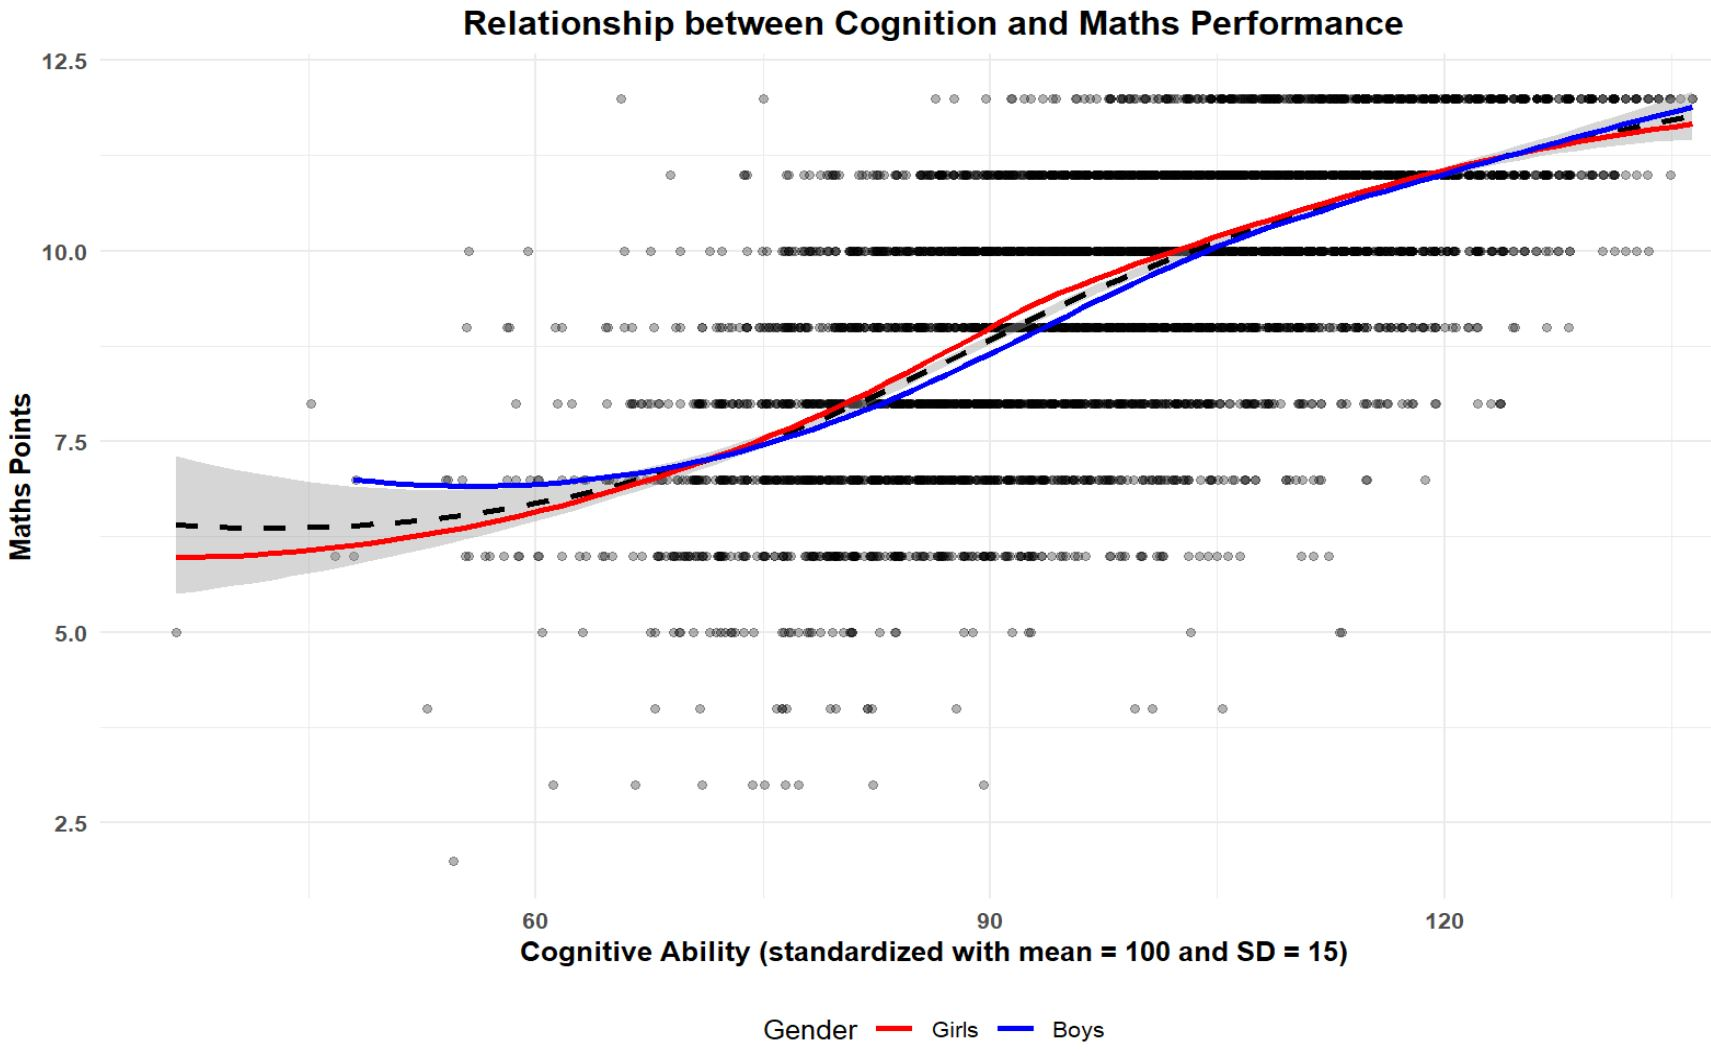
\includegraphics[width=1\linewidth]{production_function_maths_cog.JPG}
    \caption{Figure \ref{fig:cog_maths} demonstrates a strong positive relationship between cognitive ability and Maths performance for both genders. The cognitive ability measure is standardized with a mean of 100 and a standard deviation of 15. As cognitive ability increases, there is a clear upward trend in Maths performance (proxied by points). This relationship appears to be slightly stronger for boys at higher and lower cognitive ability levels. Overall it seems that the relationship between cognitive ability and Maths performance is not linear, especially for girls.}
    \label{fig:cog_maths}
\end{figure*}

\begin{figure*}[ht] 
    \centering
    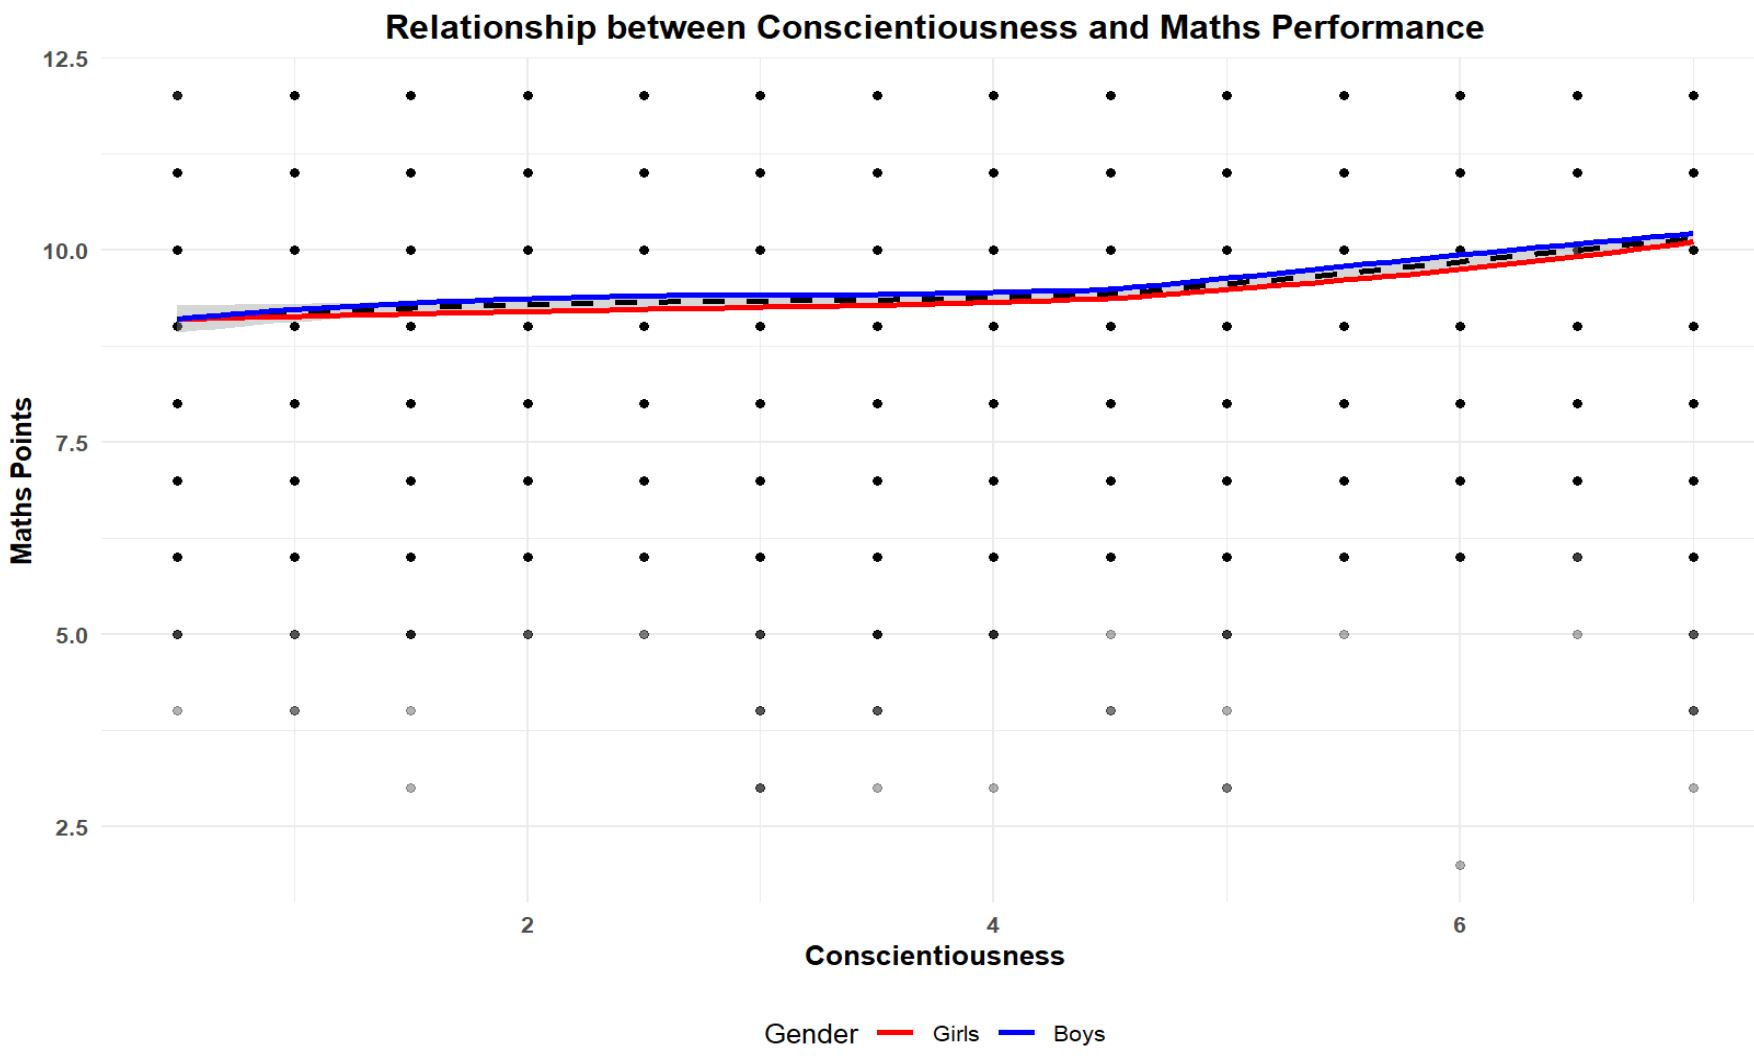
\includegraphics[width=1\linewidth]{production_function_maths_cons.JPG}
    \caption{Figure \ref{fig:con_maths} demonstrates a positive relationship between Conscientiousness and Maths performance. The curve for boys is steeper at higher levels of Conscientiousness, which indicates that high levels of Conscientiousness might be particularly beneficial for boys' Maths performance.}
    \label{fig:con_maths}
\end{figure*}

\begin{figure*}[ht] 
    \centering
    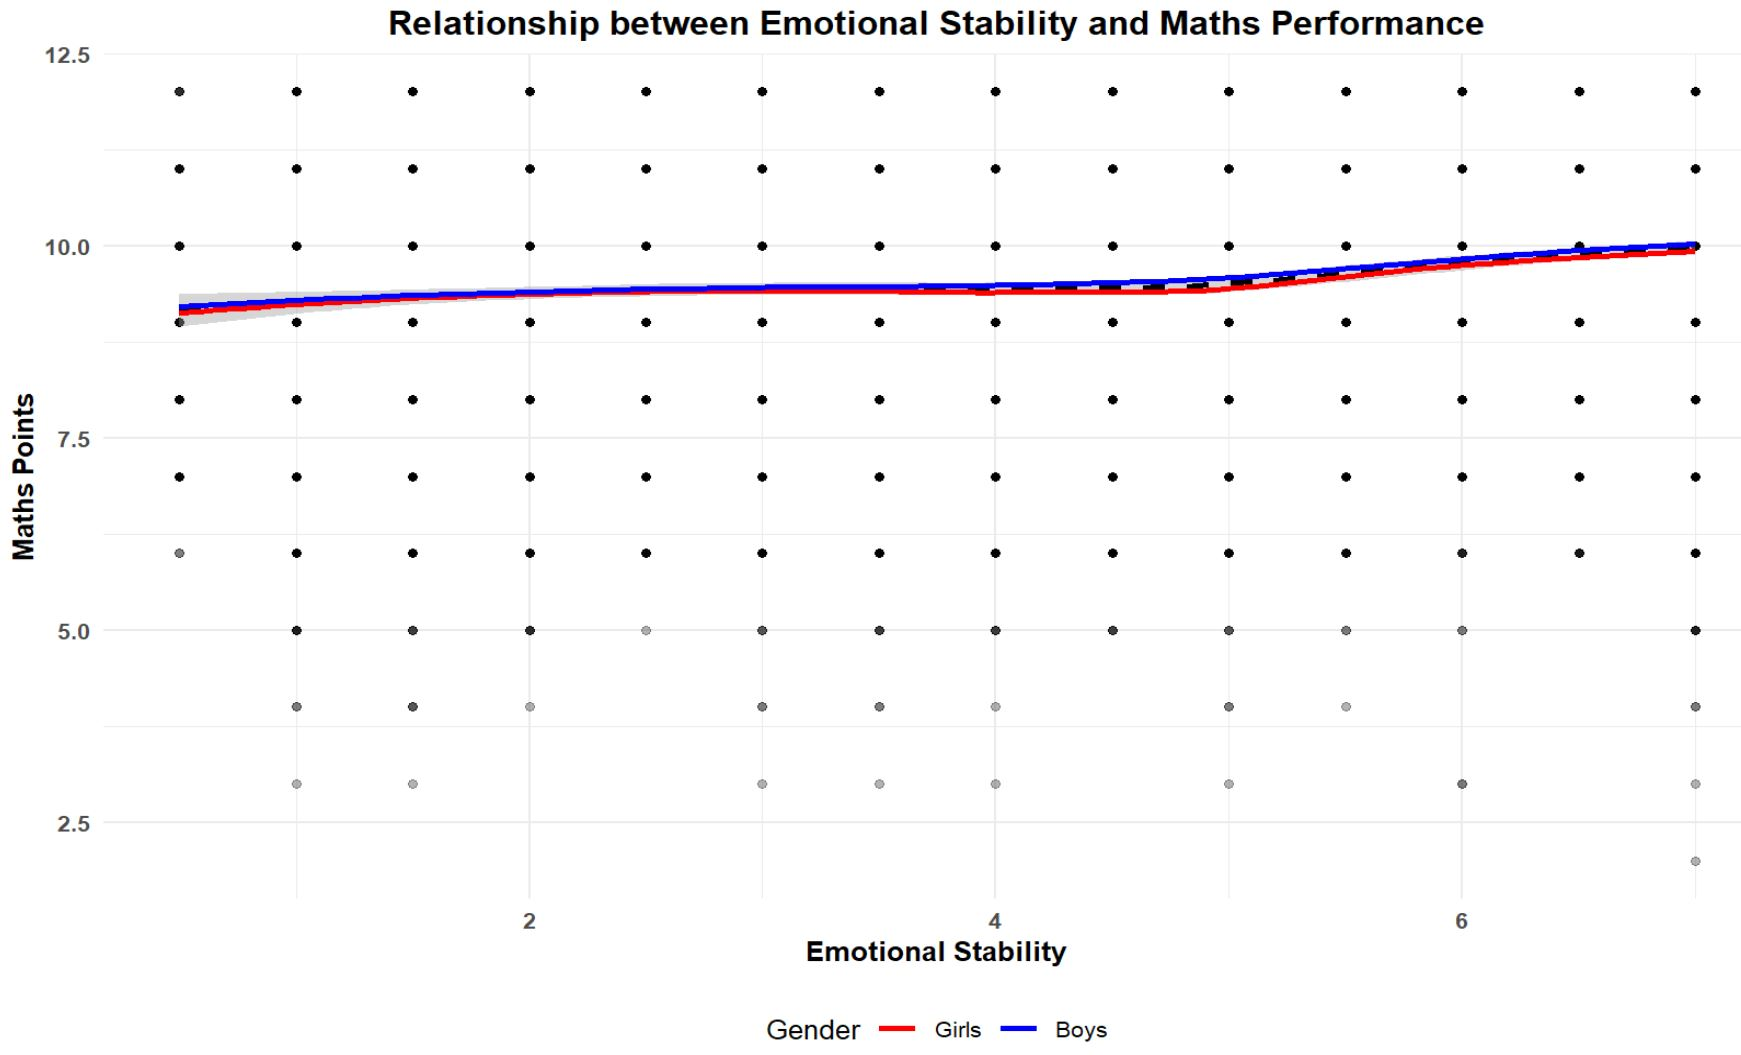
\includegraphics[width=1\linewidth]{production_function_maths_emostab.JPG}
    \caption{Figure \ref{fig:emostab_maths} illustrates a slightly positive relationship between Emotional Stability and Maths performance for higher levels of Emotional Stability. The curve is slightly steeper for boys, which suggests that Emotional Stability has a somewhat stronger impact on boys' Maths performance compared to girls'.}
    \label{fig:emostab_maths}
\end{figure*}

\begin{figure*}[ht] 
    \centering
    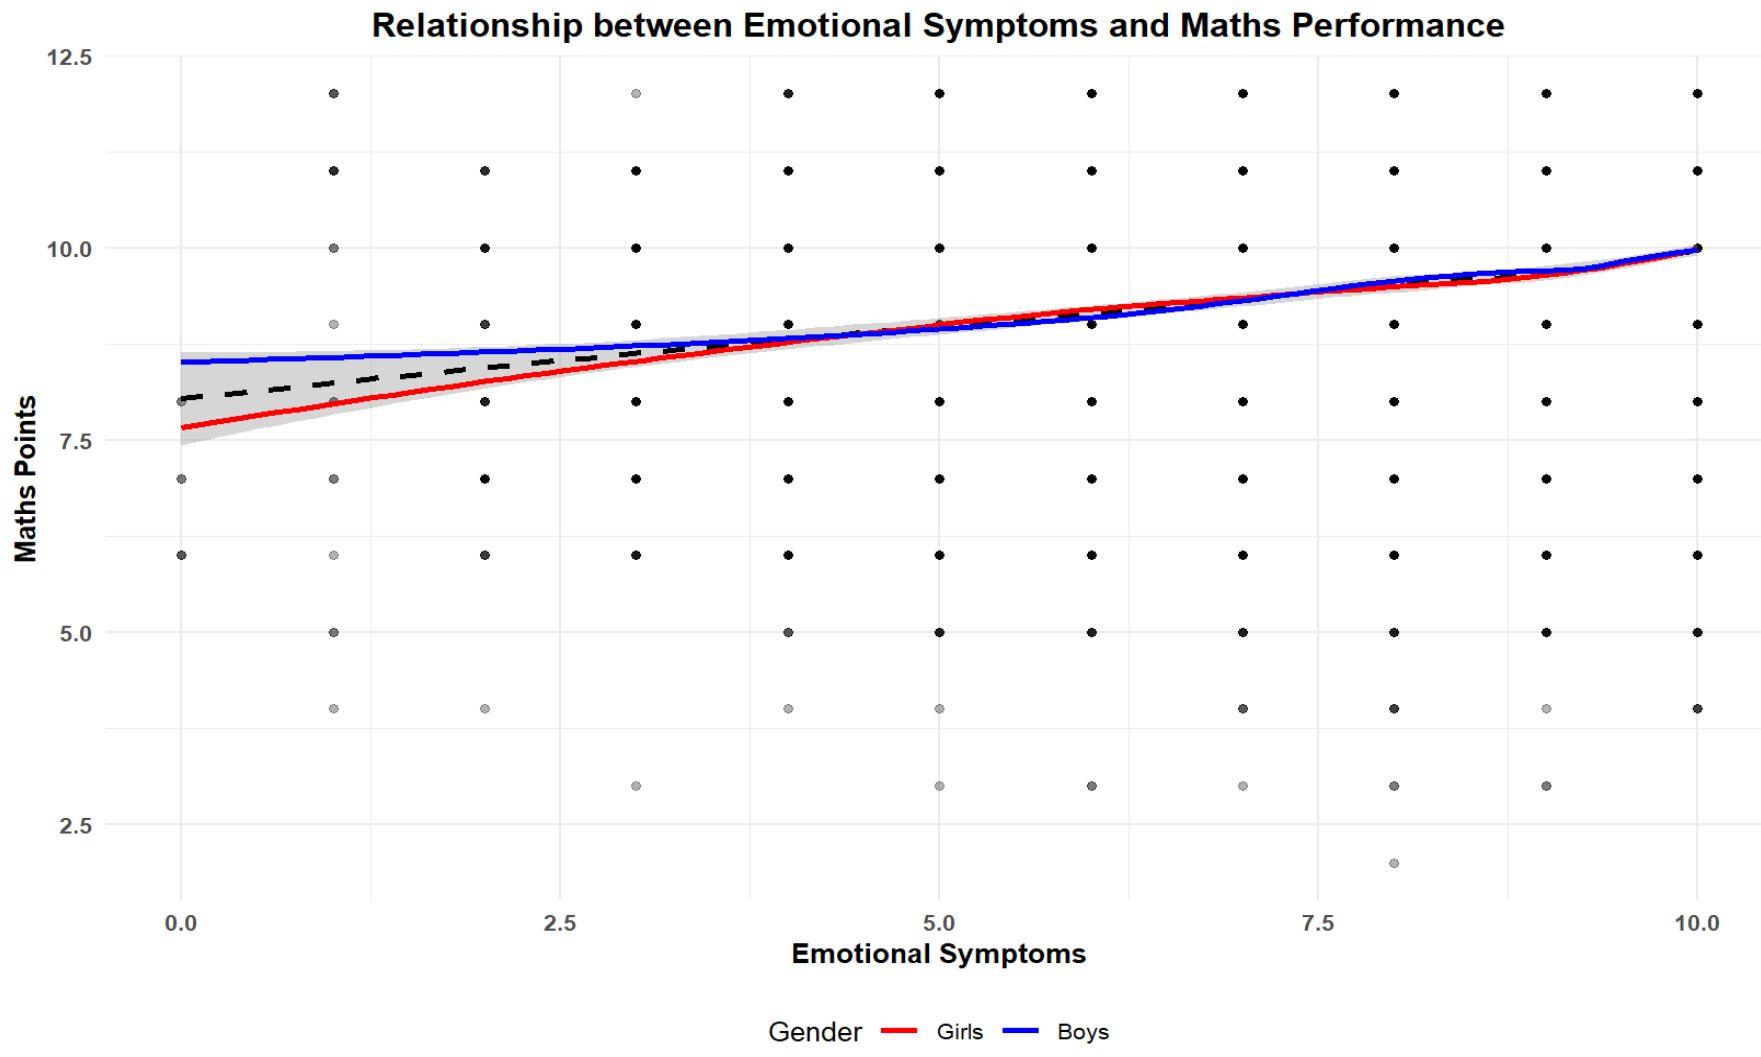
\includegraphics[width=1\linewidth]{production_function_maths_emosym.JPG}
    \caption{Figure \ref{fig:emosym_maths} shows a slight positive relationship between Emotional Symptoms and Maths performance. There appears to be a small gender difference in this relationship at the lower end (where boys and girls have lower levels of Emotional Symptoms), which indicates that lower levels of Emotional Symptoms affect girls' Maths performance more than boys'.}
    \label{fig:emosym_maths}
\end{figure*}

\begin{figure*}[ht] 
    \centering
    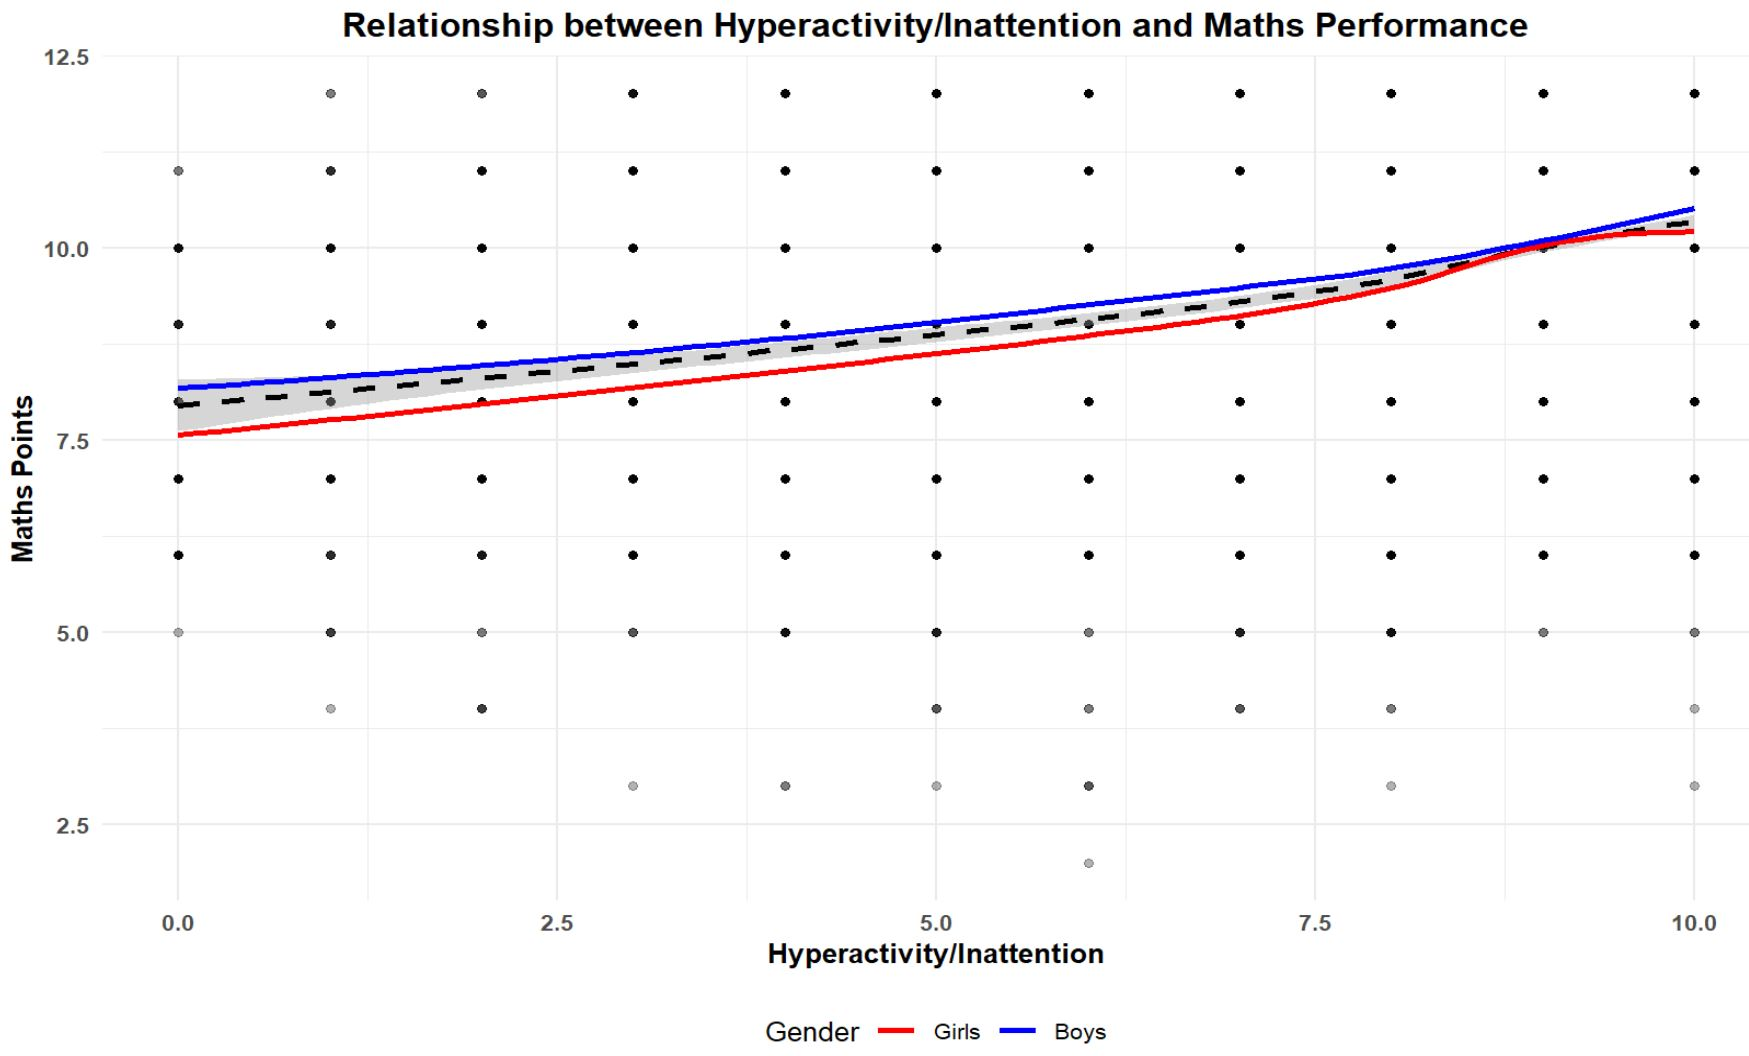
\includegraphics[width=1\linewidth]{production_function_maths_hyper.JPG}
    \caption{Figure \ref{fig:hyper_maths} reveals a positive relationship between Hyperactivity/Inattention and Maths performance (the original SDQ sub-scale was inverted, so low levels of Hyperactivity/Inattention in the graph mean lower levels of control, balance, and attention). Higher levels of Hyperactivity/Inattention (or higher levels of attention and control) are associated with higher Maths performance (proxied by points). This effect seems to be more pronounced for boys, especially at higher levels of Hyperactivity/Inattention, which suggests that interventions targeting attention control might be particularly beneficial for boys' performance in Maths.}
    \label{fig:hyper_maths}
\end{figure*}

\begin{figure*}[ht] 
    \centering
    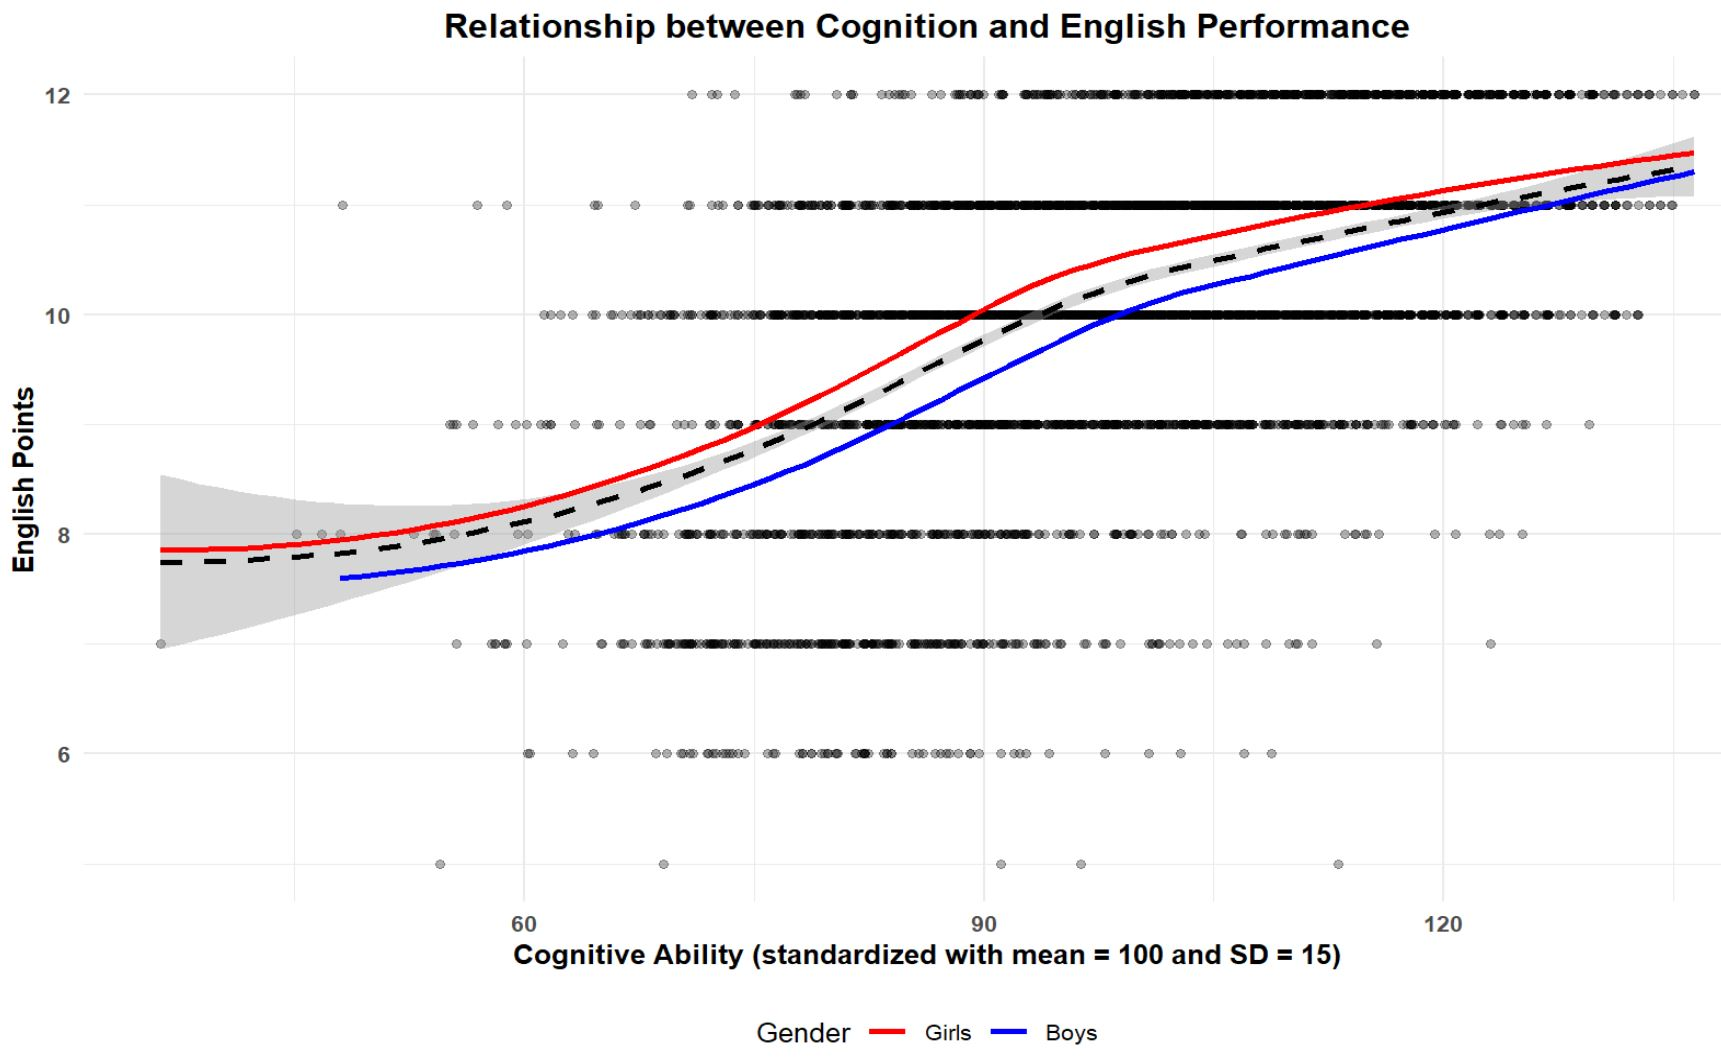
\includegraphics[width=1\linewidth]{production_function_english_cog.JPG}
    \caption{Figure \ref{fig:cog_English} shows a strong positive relationship between cognitive ability and English performance. Notably, girls appear to perform better than boys across all levels of cognitive ability, suggesting a persistent gender gap in English performance that is not fully explained by cognitive ability.}
    \label{fig:cog_English}
\end{figure*}

\begin{figure*}[ht] 
    \centering
    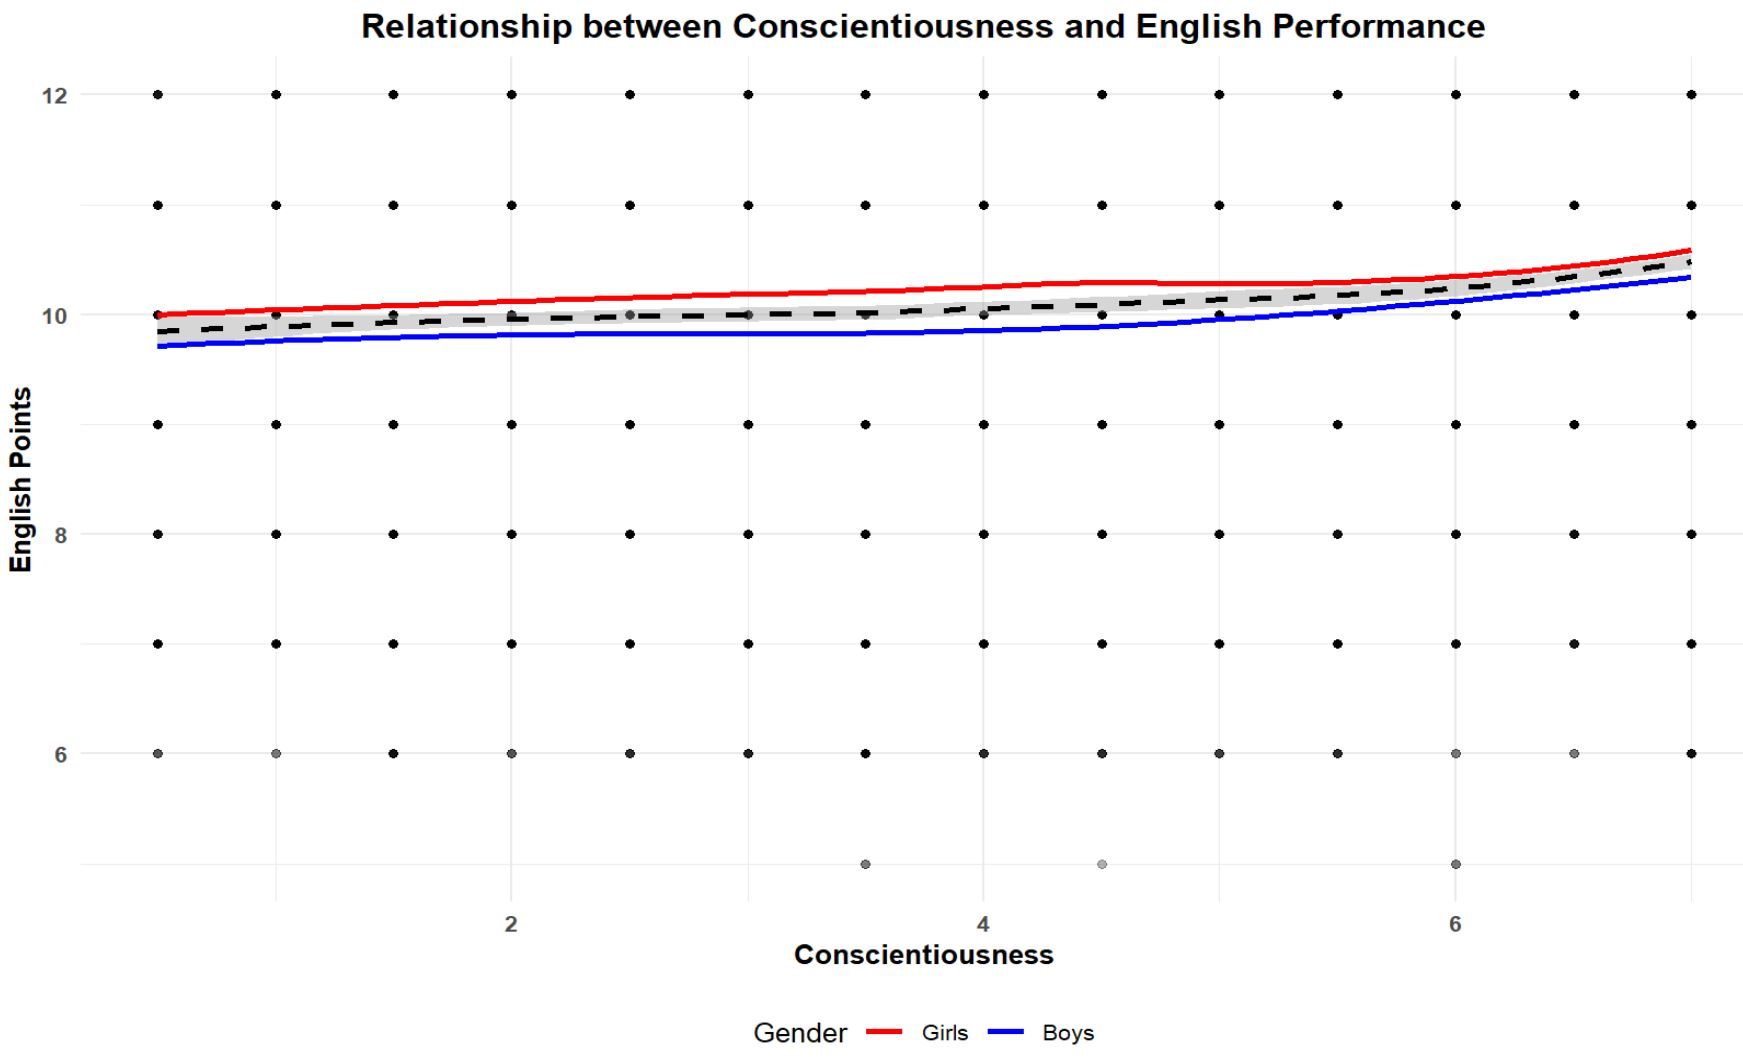
\includegraphics[width=1\linewidth]{production_function_english_cons.JPG}
    \caption{Figure \ref{fig:con_English} exhibits a positive relationship between Conscientiousness and English performance. As with Maths, boys show a slightly steeper curve at higher levels of Conscientiousness, suggesting that high Conscientiousness might be particularly beneficial for boys' English performance, and it would help close the gender achievement gap.}
    \label{fig:con_English}
\end{figure*}

\begin{figure*}[ht] 
    \centering
    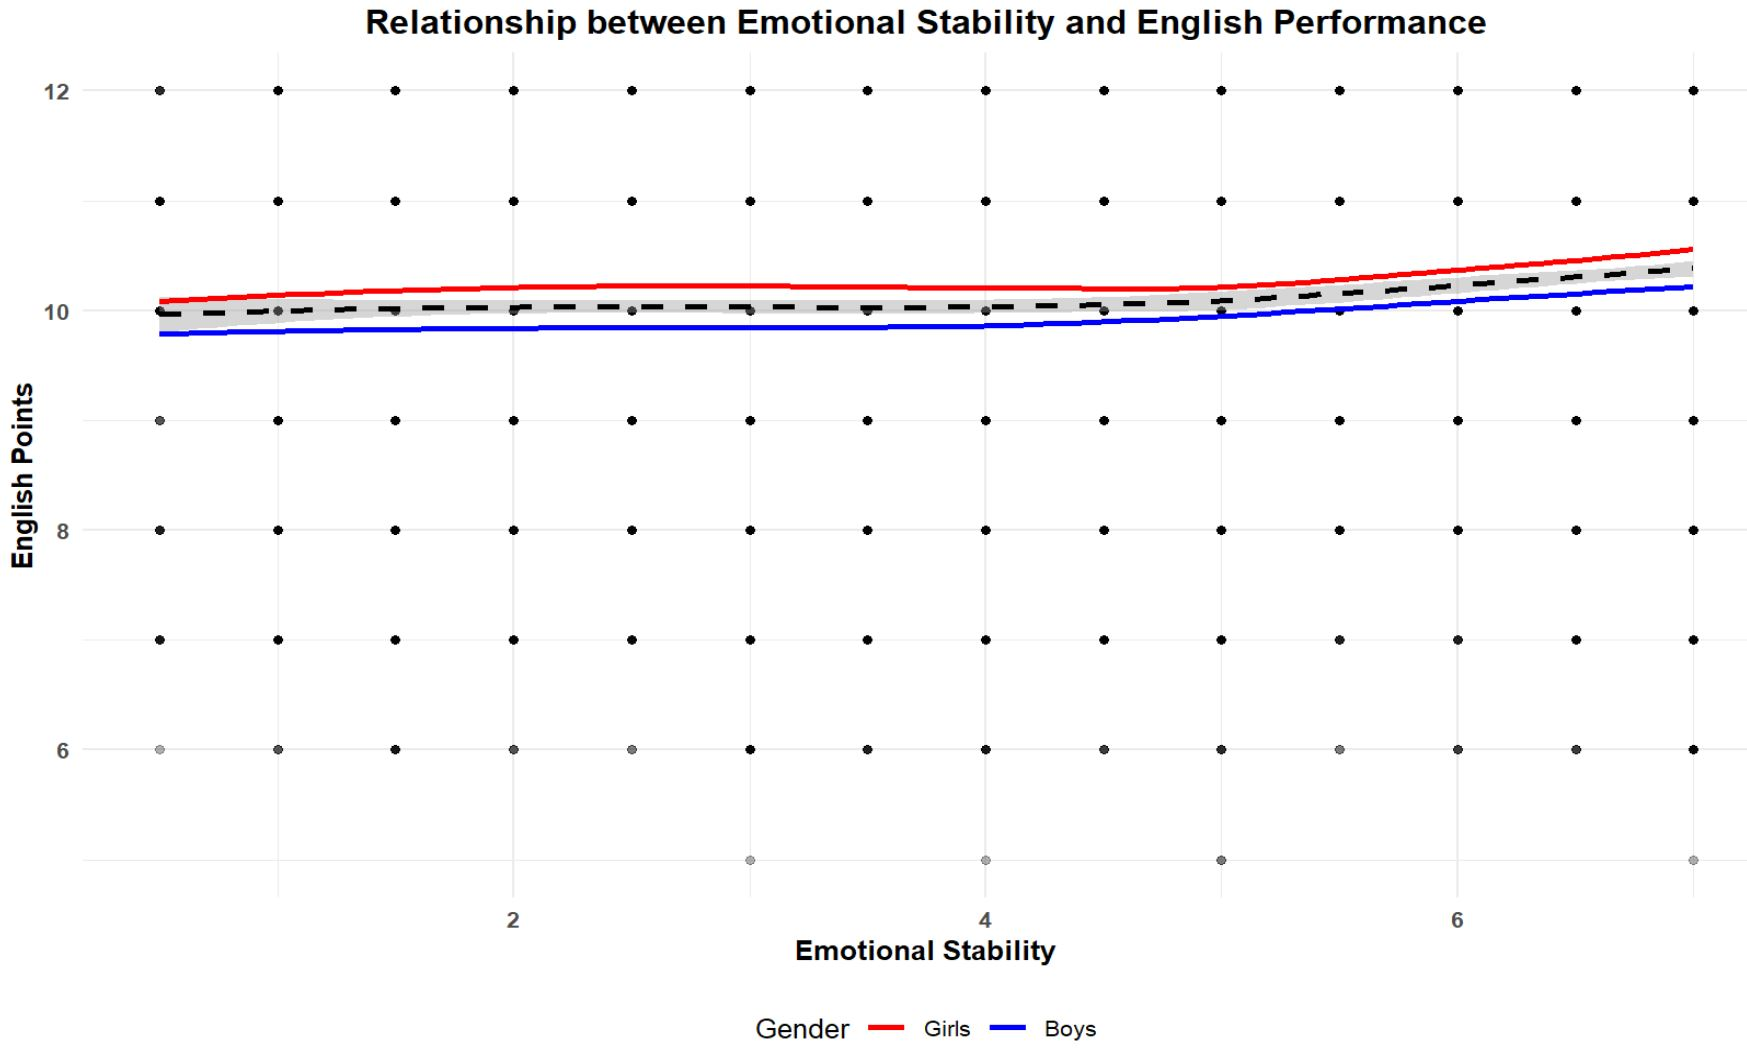
\includegraphics[width=1\linewidth]{production_function_english_emostab.JPG}
    \caption{Figure \ref{fig:emostab_English} demonstrates a positive relationship between Emotional Stability and English performance. Boys, again, show a slightly steeper curve, indicating that Emotional Stability might have a marginally stronger impact on boys' English performance.}
    \label{fig:emostab_English}
\end{figure*}

\begin{figure*}[ht] 
    \centering
    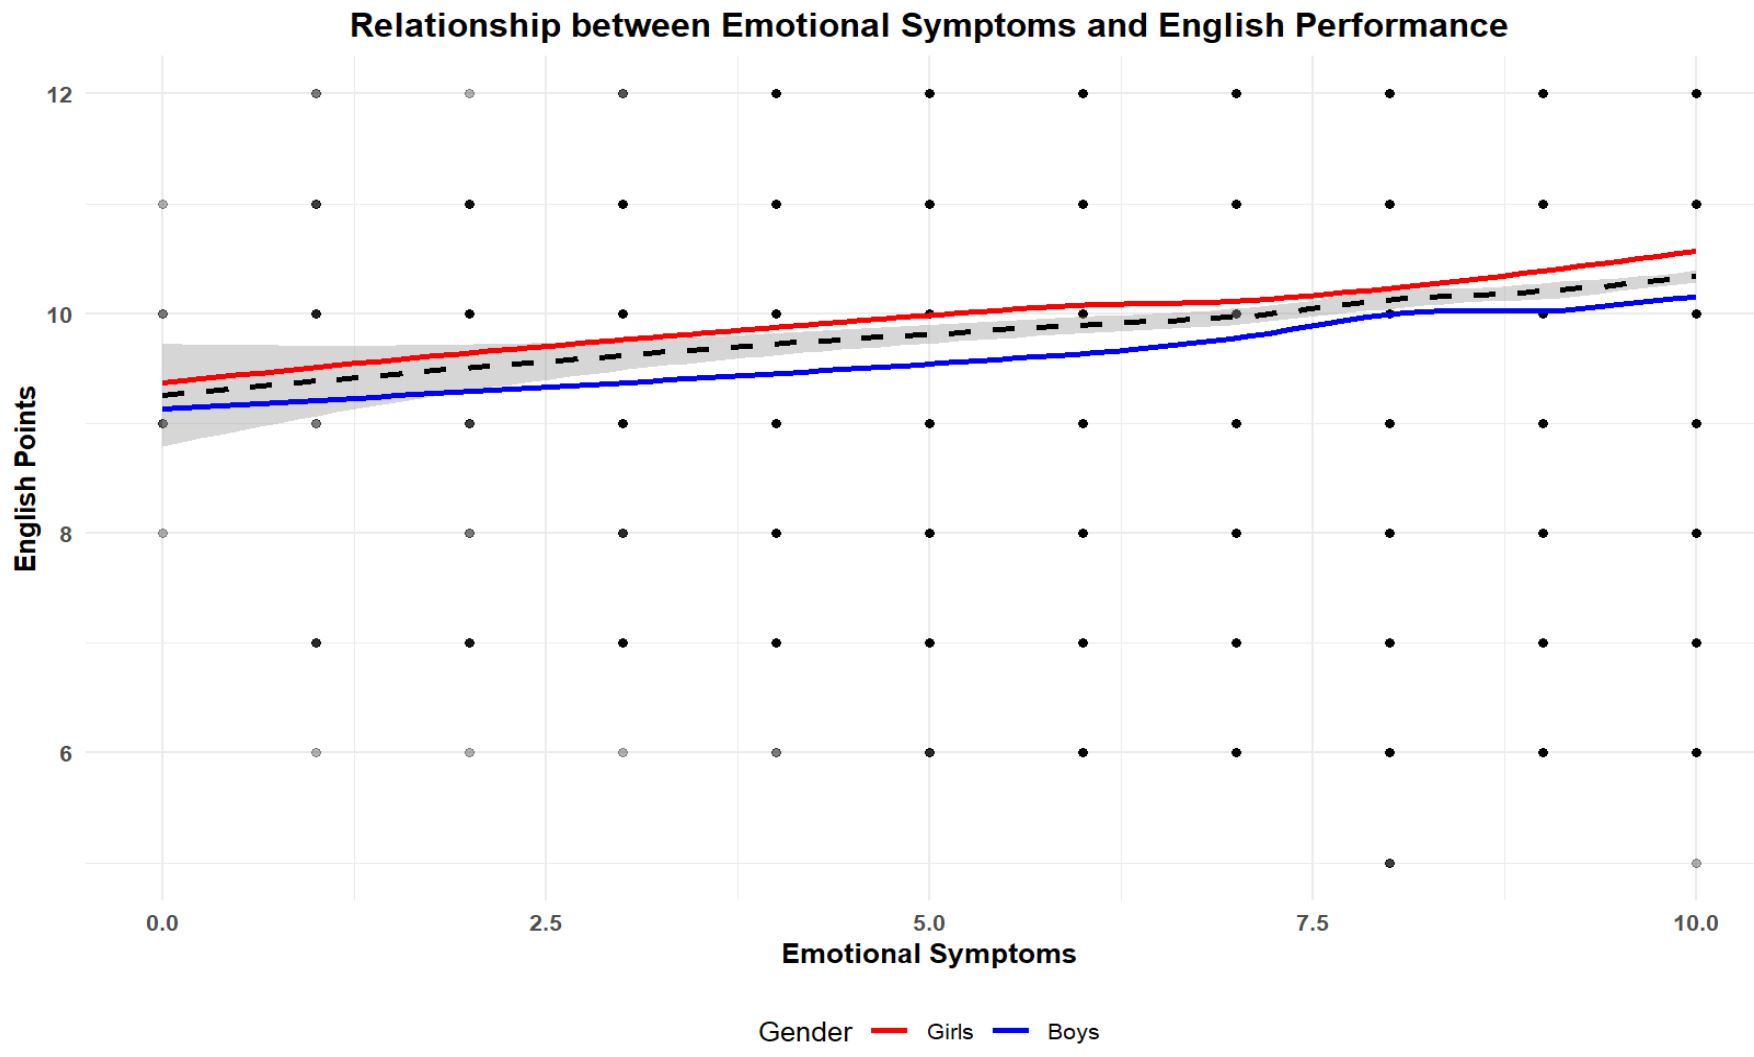
\includegraphics[width=1\linewidth]{production_function_english_emosym.JPG}
    \caption{Figure \ref{fig:emosym_English} reveals a positive relationship between Emotional Symptoms and English performance, with a small, but apparent, gender difference (it is more pronounced for girls).}
    \label{fig:emosym_English}
\end{figure*}

\begin{figure*}[ht] 
    \centering
    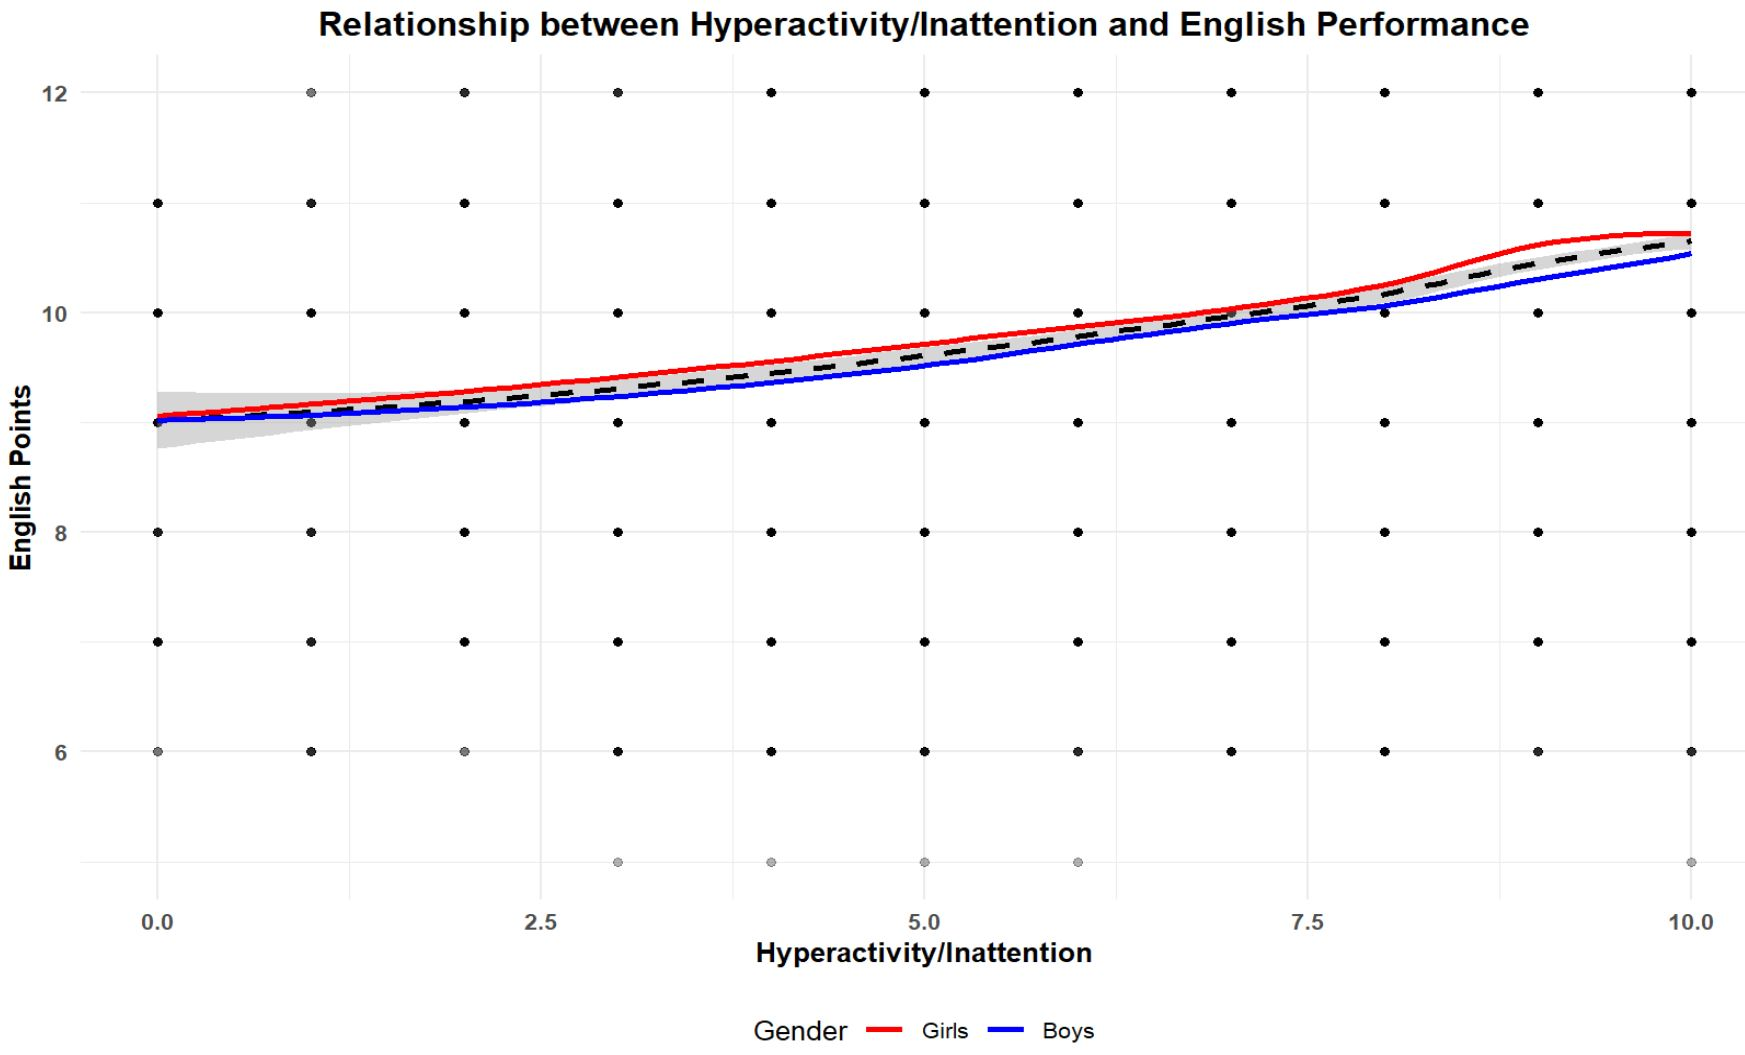
\includegraphics[width=1\linewidth]{production_function_english_hyper.JPG}
    \caption{Figure \ref{fig:hyper_English} displays a positive relationship between Hyperactivity/Inattention and English performance, similar to Maths (where the original SDQ sub-scale was inverted, so low levels of Hyperactivity/Inattention in the graph mean lower levels of control, balance, and attention). Higher levels of Hyperactivity/Inattention (or higher levels of attention and control) are also associated with higher English performance (proxied by points) especially for boys at higher levels of Hyperactivity/Inattention. This consistency across subjects highlights the importance of addressing attention-related issues, particularly for boys.}
    \label{fig:hyper_English}
\end{figure*}

4. Visualization of cognitive and noncognitive factors in academic performance: Because we have seen time and time again in the main text that the relationship between cognitive and noncognitive factors is potentially nonlinear and heterogeneous in levels and genders, I plotted each independent variable considered significant against the dependent variable. All figures use a scatter plot to represent individual data points, with LOESS (locally weighted smoothing) lines overlaid to show general trends.

\clearpage
\printbibliography

\end{document}